\documentclass{tufte-book}

\hypersetup{colorlinks}

\renewcommand{\maketitlepage}[0]{%
  \cleardoublepage%
  {%
  \sffamily%
  \begin{fullwidth}%
  \fontsize{18}{20}\selectfont\par\noindent\textcolor{darkgray}{\allcaps{\thanklessauthor}}%
  \vspace{9pc}%
%  \vspace{11.5pc}%
%  \fontsize{24}{40}\selectfont\par\noindent\textcolor{darkgray}{\allcaps{\thanklesstitle}}%
  \fontsize{32}{40}\selectfont\par\noindent\textcolor{darkgray}{\allcaps{\thanklesstitle}}%
  \vfill%
    \fontsize{18}{40}\selectfont\par\noindent\textcolor{darkgray}{\allcaps{numerical solutions using}}%
    \fontsize{18}{40}\selectfont\par\noindent\textcolor{darkgray}{\allcaps{the Portable, Extensible Toolkit for Scientific computation} v.~3.5}%
  \vfill%
  \fontsize{14}{16}\selectfont\par\noindent\allcaps{\thanklesspublisher}%
  \end{fullwidth}%
  }
  \thispagestyle{empty}%
  \clearpage%
}

\title[PETSc for PDEs]{PETSc \\ for \\ Partial \\ Differential \\ Equations}

\author{Ed Bueler}
\publisher{Maybe Someday a Publisher of This Book}

\date{\today}

\usepackage{booktabs} % for nicely-typeset tabular material
\usepackage{verbatim} % for "comment" environment
\usepackage{xspace}
%\usepackage{underscore} % causes "Missing \endcsname inserted" error?
\usepackage{fancyvrb}
\usepackage{graphicx}
\usepackage{amsmath,amssymb,amsthm,bm}
\usepackage{tikz}

\usetikzlibrary{arrows,decorations.markings,fadings}

%\usepackage[subtle,floats]{savetrees}

% macros

\theoremstyle{definition}
\newtheorem*{example}{{\color{cyan} Example}}

\newcommand{\trueinput}[2]{
\VerbatimInput[frame=single,framesep=3mm,label=\fbox{\normalsize \textsl{\,#1\,}},fontfamily=courier,fontsize=\footnotesize]{#2}
}

%\inputfromline{FULLPATH}{FILENAME}{CAPTION}{FIRSTLINE}{LABEL}
\newcommand{\inputfromline}[5]{
\vspace{0.8cm}
\let\FancyVerbStartString\relax
\let\FancyVerbStopString\relax
\begin{minipage}[l]{1.25\textwidth}
\VerbatimInput[frame=single,%
               framesep=3mm,%
               label=\fbox{\small \textsl{\,#2\,}},%
               fontfamily=courier,%
               fontsize=\footnotesize,%
               firstline=#4]{#1}
\end{minipage}
\vspace{0.5cm}

\begin{marginfigure}[1.0cm]
\caption{#3}
\label{#5}
\end{marginfigure}

\vspace{1.5cm}
}

\newcommand{\inputwhole}[4]{\inputfromline{#1}{#2}{#3}{1}{#4}}

%\cinputraw{FULLPATH}{FILENAME}{CAPTION}{PARTSTRING}{STARTSTRING}{STOPSTRING}{LABEL}
\newcommand{\cinputraw}[7]{
\newcommand*\FancyVerbStartString{#5}
\newcommand*\FancyVerbStopString{#6}
\vspace{0.8cm}
\begin{minipage}[l]{1.25\textwidth}
\VerbatimInput[frame=single,%
               framesep=3mm,%
               label=\fbox{\small \textsl{\,#2\,}#4},%
               fontfamily=courier,%
               fontsize=\footnotesize]{#1}
\end{minipage}
\vspace{0.5cm}

\begin{marginfigure}[1.0cm]
\caption{#3}
\label{#7}
\end{marginfigure}

\vspace{1.5cm}
\let\FancyVerbStartString\relax
\let\FancyVerbStopString\relax
}

\newcommand{\cinput}[5]{%
    \cinputraw{cstrip/#1}{#1}{#2}{}{#3}{#4}{#5}}
\newcommand{\cinputnostrip}[5]{%
    \cinputraw{../c/#1}{#1}{#2}{}{#3}{#4}{#5}}

\newcommand{\cinputpart}[6]{%
    \cinputraw{cstrip/#1}{#1}{#2}{\quad \textbf{part #3}}{#4}{#5}{#6}}
\newcommand{\cinputpartnostrip}[6]{%
    \cinputraw{../c/#1}{#1}{#2}{\quad \textbf{part #3}}{#4}{#5}{#6}}

\newcommand{\caveat}[1]{\marginnote{\textsc{Where we stand:}\\  #1}}

% Prints an epigraph and speaker in sans serif, all-caps type.
\newcommand{\openepigraph}[2]{%
  %\sffamily\fontsize{14}{16}\selectfont
  \begin{fullwidth}
  \sffamily\large
  \begin{doublespace}
  \noindent\allcaps{#1}\\% epigraph
  \noindent \Large \allcaps{#2}% author
  \end{doublespace}
  \end{fullwidth}
}

\newcommand{\monthyear}{%
  \ifcase\month\or January\or February\or March\or April\or May\or June\or
  July\or August\or September\or October\or November\or
  December\fi\space\number\year
}

\newcommand{\bA}{\mathbf{A}}
\newcommand{\bB}{\mathbf{B}}
\newcommand{\bE}{\mathbf{E}}
\newcommand{\bF}{\mathbf{F}}
\newcommand{\bJ}{\mathbf{J}}

\newcommand{\bb}{\mathbf{b}}
\newcommand{\bc}{\mathbf{c}}
\newcommand{\bn}{\mathbf{n}}
\newcommand{\bq}{\mathbf{q}}
\newcommand{\br}{\mathbf{r}}
\newcommand{\bu}{\mathbf{u}}
\newcommand{\bv}{\mathbf{v}}
\newcommand{\bw}{\mathbf{w}}
\newcommand{\bx}{\mathbf{x}}
\newcommand{\by}{\mathbf{y}}

\newcommand{\CC}{\mathbb{C}}
\newcommand{\RR}{\mathbb{R}}
\newcommand{\ZZ}{\mathbb{Z}}

\newcommand{\X}{\times}  % for nonzero entries in matrices
\newcommand{\redX}{{\color{red} \bm{\underline{\X}}}}
\newcommand{\blueX}{{\color{blue} \bm{\underline{\X}}}}

\newcommand{\XX}{$\bm{\times}$}  % for ticks in tables
\newcommand{\gX}{{\color{Gray} $\times$}}

\newcommand{\eps}{\epsilon}
\newcommand{\lam}{\lambda}
\newcommand{\lap}{\triangle}

\newcommand{\Div}{\ensuremath{\nabla\cdot}}
\newcommand{\Curl}{\ensuremath{\nabla\times}}
\newcommand{\grad}{\nabla}

\newcommand{\ip}[2]{\ensuremath{\left<#1,#2\right>}}

\newcommand{\cond}{\operatorname{cond}}
\newcommand{\onull}{\operatorname{null}}
\newcommand{\rank}{\operatorname{rank}}
\newcommand{\range}{\operatorname{range}}
\newcommand{\Span}{\operatorname{span}}

\renewcommand{\Re}{\operatorname{Re}}
\renewcommand{\Im}{\operatorname{Im}}

\newcommand{\Th}{\mathcal{T}_h}
\newcommand{\Pone}{\mathbf{P}_1}

\newcommand{\Matlab}{\textsc{Matlab}\xspace}
\newcommand{\Triangle}{\textsc{triangle}\xspace}
\newcommand{\MPI}{\textsc{MPI}\xspace}

\newcommand{\PETSc}{\textsc{PETSc}\xspace}

\newcommand{\pDM}{\texttt{DM}\xspace}

\newcommand{\pDMDA}{\texttt{DMDA}\xspace}
\newcommand{\pDMPlex}{\texttt{DMPlex}\xspace}
\newcommand{\pKSP}{\texttt{KSP}\xspace}
\newcommand{\pSNES}{\texttt{SNES}\xspace}
\newcommand{\pTS}{\texttt{TS}\xspace}

\newcommand{\pMat}{\texttt{Mat}\xspace}
\newcommand{\pMats}{\texttt{Mat}s\xspace}

\newcommand{\pVec}{\texttt{Vec}\xspace}
\newcommand{\pVecs}{\texttt{Vec}s\xspace}

%\renewcommand\floatpagefraction{.9}  %???

% eventually this is a good idea:
%\usepackage{makeidx}
%\makeindex

\begin{document}

\begin{comment}
% epigraph page first
\newpage\thispagestyle{empty}
\openepigraph{%
\dots when there are disputes among persons, we can simply say: Let us calculate, without further ado, to see who is right.
}{Gottfried Wilhelm Leibniz}
\vfill
\openepigraph{%
Developing parallel, nontrivial PDE solvers that deliver high performance is still difficult and requires months (or even years) of concentrated effort.  PETSc is a toolkit that can ease these difficulties and reduce the development time, but it is not a black-box PDE solver, nor a silver bullet
}{Barry Smith}
\vfill
\openepigraph{%
Tufte's style is known for its extensive use of sidenotes, tight integration of graphics with text, and well-set typography.
}{The Tufte-LaTeX\ Developers}
\vfill

\frontmatter
\end{comment}

\maketitle

% v.4 copyright page
\newpage
\begin{fullwidth}
~\vfill
\thispagestyle{empty}
\setlength{\parindent}{0pt}
\setlength{\parskip}{\baselineskip}
Copyright \copyright\ \the\year\ \thanklessauthor

\par\smallcaps{Published by \thanklesspublisher}

%\par  [license here] I have no idea if I should license this at this stage

\par\textit{First printing, \monthyear}
\end{fullwidth}

\tableofcontents

\begin{comment}
% dedication
\cleardoublepage
~\vfill
\begin{doublespace}
\noindent\fontsize{18}{22}\selectfont\itshape
\nohyphenation
Thanks to \mbox{Jed Brown} and \mbox{Constantine Khroulev}, fellow students, and gurus.
\end{doublespace}
\vfill
\end{comment}

%%%%%%%%%%

\chapter{Why this book?}


You've taken a mathematics course or two in partial differential equations (PDEs).  Somewhere you picked up a bit of coding in C; perhaps you write C code every day.\sidenote{You know that ``API'' stands for ``application program interface,'' for example.}  You've also written various short scripts in \Matlab or python, and you've even tried solving PDEs numerically.  But \emph{now you want it all in parallel on big problems}.  This book is for you and me.

\section{\PETSc?}

The Portable, Extensible Toolkit for Scientific computing (\PETSc\sidenote{Say it ``pets sea.''}) \citep{petsc-user-ref} is an open-source, mathematical software library built on top of the standard software layer for large-scale parallel computation, the Message Passing Interface (MPI) \citep{Groppetal1999}.  Thus \PETSc is a framework for solving problems like PDS at ``large scale,'' that is, at high resolution and on supercomputers with hundreds to millions of cores.

\PETSc is not particularly new.  Version 2.0, the first version to make an impact in the scientific computing world, was built in 1994.  A well-known monograph \citet{Smithetal1996}\sidenote{B.~Smith, P.~Bjorstad, and W.~Gropp. \emph{Domain decomposition: parallel multilevel methods for elliptic partial differential equations}. Cambridge
University Press, 1996} uses \PETSc 2.0 for scalable solutions of linear partial differential equations (PDEs).  That book focusses on pre-conditioned iterative linear solvers.  For example, domain decomposition methods like additive Schwarz are shown to scalably solve the Poisson equation on irregular domains and fine meshes in parallel.

But \PETSc is now at version 3.5.\sidenote{Version 3.5.2 is current in September 2014.  The stable homepage URL for PETSc, including download and installation instructions, is at \href{http://www.mcs.anl.gov/petsc/index.html}{www.mcs.anl.gov/petsc}.}  It has evolved into a more powerful toolbox with a much richer API.

Typical examples and applications now solve nonlinear PDEs at scale.  The \PETSc strategy is to compose Newton's method and mesh topology tools with a run-time chooseable selection of preconditioners and iterative linear solvers.  The nonlinear and multilevel-related parts of the \PETSc API are now highly-visible to users of \PETSc 3.5.  ``Multiphysics problems''\sidenote{This buzzword just refers to a diverse system of coupled PDEs with nontrivial scalings among the variables.  But that is a concept that \emph{needs} a buzzword.} are now within reach.  \PETSc may not be a silver bullet, but users see powerful tools, beyond linear algebra, to solve hard problems.

On the other hand, \PETSc is notoriously complicated.  Twenty years have passed since \PETSc version 2.0.  Perhaps a new book is needed.

\section{The goals of this book}

This book is about numerically solving linear and nonlinear PDEs in 2 or 3 spatial variables by writing C code that directly calls \PETSc.  This book tries to both explain the ideas directly, and illustrate them through example codes.  The example codes come with enough background information so that readers can use them as a basis for further developments.  Demonstrated scalability is the goal, so runtime options are explained and compared.

This book does not replace the \PETSc \emph{User's Manual}.  Indeed, the current book assumes you want to solve PDEs, while there are many other uses of \PETSc.

This book is written from the conviction that better access to common knowledge among experts advances scientific computing as a discipline.  In fact, accessing common knowledge advances the discipline faster than does original research among the experts.  Said another way, I hope that an expert in \PETSc will say about this book's content that ``I knew all that'' \emph{and} that ``this book is a fast on-ramp to what I already know.''

\section{What I need from you, the reader}

To make sense of this book, some of the mathematical theory\sidenote{\citep{Evans} is recommended, but not really a prerequisite.} of PDEs must be familiar.  I will also assume some nebulous, and hard to define, practical intuition about PDE problems, including exposure to nonlinear ones.\sidenote{\citep{Ockendonetal2003} is recommended.}  Of course, all applied mathematicians, distinctly including this author, are wanting when it comes to injesting the mathematical theory of, and building intuition for, nonlinear PDEs.

Multiple numerical discretization paradigms for PDEs will arise in this book.  At least one such numerical approach to PDEs should be in the reader's toolbox.  This background might be based on the finite element method (FEM) \citep{Braess,Elmanetal2005}, finite differences \citep{MortonMayers}, finite volumes \citep{LeVeque}, or spectral methods \citep{KarniadakisSherwin,Trefethen}.  Exposure to multigrid ideas \citep{Briggsetal2000} would be helpful, but these concepts will be reviewed.  Numerical ideas from linear algebra \citep{Greenbaum1997,TrefethenBau} will also appear, often with only a brief introduction.

Starting in Chapter 3 I will assume that you are at least a bit interested in applying the finite element method (FEM) on unstructured grids, though not at the exclusion of structured approaches.  The basics of the FEM method will be reviewed, but the reader must also bring some background understanding of this nontrivial topic.  Perhaps the weak form of a PDE, and the idea of assembling the systems of equations element-by-element, are rusty topics, but they should be in there somewhere.

Searching in the \PETSc HTML manual pages should be the reader's first resort for resolving compile-time errors, or for exposing the \PETSc API.  However, the reader should also review the \PETSc \emph{Users Manual}.  That \emph{Manual} explains why the API is designed in the way it is.


\section{There is much that this book does NOT do}

This book\begin{itemize}
\item  does not help you install \PETSc,
\item  does not use Fortran or C++, and all examples are in C,\sidenote{We use ANSI C99 features.}
\item  does not help with most of the many packages \PETSc links to,
\item  does not do a complete job of teaching the finite element method or any other discretization paradigm for PDEs,
\item  does not consider spatial dimensions except 2 and 3,
\item  does not prove anything,\sidenote{We do give evidence for convergence and scalability when possible.}
\item  does not care whether its numerical solutions are good models of physical problems, and
\item  does not adequately cover what is known about nonlinear PDEs, much less what is not known.
\end{itemize}


\mainmatter

%%%%%%%%%


\chapter{Getting started with PETSc}
\label{chap:getstarted}

\section{A code that does almost nothing, but in parallel}

The purpose of the \PETSc library is to help you solve scientific and engineering problems, on multi-processor computers.  As \PETSc is built ``on top of'' the Message Passing Interface (MPI; \citep{Groppetal1999}) library, some of the MPI flavor comes through.  Therefore we start with an introductory \PETSc code which calls MPI for some basic tasks.

This code \texttt{e.c}, shown in its entirety in Figure \ref{code:e}, approximates Euler's constant
\begin{equation}
e = \sum_{n = 0}^\infty \frac{1}{n!} \approx 2.718281828 \label{introeseries}
\end{equation}
It does the computation in a distributed manner by computing one term of the infinite series on each process, giving a better estimate of $e$ when run on more MPI processes. While this is a silly use of \PETSc, it is an easy-to-understand parallel computation.

As with any C source code, \texttt{e.c} has a function called \texttt{main()} which takes inputs from the command line, namely \texttt{argc} and \texttt{argv},\sidenote{Here \texttt{argc} is an \texttt{int} holding the argument count and \texttt{argv} is an array of strings (i.e.~type \texttt{char**}) holding the command line including all arguments.  In all our codes we simply pass these arguments to \PETSc through the \texttt{PetscInitialize()} method; it extracts options through this mechanism.} and which outputs an \texttt{int}.  The output is $0$ if the program succeeds.  Also like all C codes, we include needed headers.  Only \texttt{petsc.h} is needed because MPI methods are included thereby.  The substance of \texttt{e.c} is to declare some variables, do a computation on each process, and communicate the results between processes to get an estimate of $e$.

Before we can compile and run \texttt{e.c}, \PETSc must be installed.  If it is not already available, go to
\begin{quote}
\href{http://www.mcs.anl.gov/petsc/download/index.html}{\texttt{www.mcs.anl.gov/petsc/download/}}
\end{quote}
to download the source code, and then follow the instructions at
\begin{quote}
\href{http://www.mcs.anl.gov/petsc/documentation/installation.html}{\texttt{www.mcs.anl.gov/petsc/documentation/installation.html}}
\end{quote}
to install.  Be sure to run ``\texttt{make test}'' and see it pass the tests.  When \PETSc is correctly installed the environment variables \texttt{PETSC\_DIR} and \texttt{PETSC\_ARCH} point to a valid installation, and the MPI command \texttt{mpiexec} is from the same MPI installation as was used in configuring \PETSc.\sidenote{Type ``\texttt{which mpiexec}'' to find which one you are running.  You may need to modify your \texttt{PATH} environment variable to get the right \texttt{mpiexec}.}

Do the following to compile \texttt{e.c}:
\begin{cline}
$ cd p4pdes/c/ch1/
$ make e
\end{cline}
%$
Calling ``\texttt{make}'' uses \texttt{p4pdes/c/ch1/makefile}.  An extract of this makefile is shown in Figure \ref{code:ch1makefile}.  For all the codes in this book, the makefile has this form, as recommended in the \PETSc \emph{User's Manual} \citep{petsc-user-ref}.

\inputwhole{../c/ch1/e.c}{\texttt{p4pdes/c/ch1/e.c}}{Compute $e$ ith \PETSc.}{code:e}

Run the code like this:
\begin{cline}
$ ./e
e is about 1.000000000000000
rank 0 did 1 flops
\end{cline}
%$
The value $1.0$ is a very poor estimate of $e$, but this code does better with more MPI processes:
\begin{cline}
$ mpiexec -n 5 ./e
e is about 2.708333333333333
rank 0 did 0 flops
rank 4 did 3 flops
rank 2 did 1 flops
rank 3 did 2 flops
rank 1 did 0 flops
\end{cline}
%$
With $N=20$ processes, and thus $N=20$ terms in series \eqref{introeseries}, we get a good double-precision estimate:
\begin{cline}
$ mpiexec -n 20 ./e
e is about 2.718281828459045
rank 0 did 0 flops
...
\end{cline}
%$

``Double precision'' refers to the 64-bit representation of real numbers, which is the type normally aliased to \texttt{PetscReal} and \texttt{PetscScalar} inside \PETSc codes.  This representation corresponds to about 15 decimal digit accuracy \citep{TrefethenBau}.

\inputtoline{../c/ch1/makefile}{extract from \texttt{p4pdes/c/ch1/makefile}}{All our \texttt{makefile}s for \PETSc examples look like this.}{6}{code:ch1makefile}

Perhaps the reader is now worried that this book was written using a large supercomputer whereas the reader has a little laptop with only a couple of cores.  In fact these five or twenty process runs work just fine on the author's laptop.  MPI processes are created as needed, using an old feature of operating systems: multitasking.  Speedup from parallelism is another matter; we will return to it.

The main job in \texttt{e.c} is to collect the sum of the terms of series \eqref{introeseries} onto each process.  Each process computes term $1/n!$, where $n$ is returned by \texttt{MPI\_Comm\_rank()}.  More precisely, \texttt{PETSC\_COMM\_WORLD} is an MPI communicator \citep{Groppetal1999} containing all processes generated by \texttt{mpiexec} in the above calls, and $n$ is the rank of the process in this communicator.  Then a call to \texttt{MPI\_Allreduce()} does the sum and then sends it back to each process.  These direct uses of the MPI library are a part of using \PETSc because \PETSc generally avoids duplicating MPI functionality.

We print the computed estimate of $e$, but each process also prints its rank and the work it did.  The formatted print command \texttt{PetscPrintf()}, which is like \texttt{fprintf()} from the C standard library, is called twice, once with MPI communicator \texttt{PETSC\_COMM\_WORLD} and once with \texttt{PETSC\_COMM\_SELF}.  The first of these printing jobs is \emph{collective} over all processes, and thus only done once, while the second is individual to each rank.\sidenote{A process is often just called a \emph{rank} in MPI language.}  In the output the \texttt{PETSC\_COMM\_SELF} printed lines can appear in random order because the print occurs as soon as that process reaches that line.

Every \PETSc program should start and end with the commands \texttt{PetscInitialize()} and \texttt{PetscFinalize()}:
\begin{code}
PetscInitialize(&argc,&args,(char*)0,help);
... everything else goes here ...
PetscFinalize();
\end{code}
As an argument to \texttt{PetscInitialize()} we supply a \texttt{help} string.  This string is a good place to say what is the purpose of the code.  To see the help string, and a longer list of possible \PETSc options, do:
\begin{cline}
$ ./e -help
\end{cline}
%$
or
\begin{cline}
$ ./e -help | less
\end{cline}
%$
Through \texttt{-help}, \PETSc programs have a built-in help system for runtime options that is both light-weight and surprisingly-effective.  For example, to see options related to logging performance, do
\begin{cline}
$ ./e -help | grep log_
\end{cline}
%$
We will see later how to add options to our own programs so that they will be documented in the same way.

Unfortunately, \texttt{e.c} and all other \PETSc programs have error-checking clutter.  While languages other than C might help with decluttering, we are stuck with ugly lines that look like
\begin{code}
ierr = PetscCommand(...); CHKERRQ(ierr);
\end{code}
The explanation is that almost all \PETSc methods, and most user-written methods in \PETSc programs, return an \texttt{int} for error checking, with value $0$ if successful.  In the line above, \texttt{ierr} is passed to the \texttt{CHKERRQ()} macro which does nothing if \texttt{ierr == 0} but which stops the program with a ``traceback'' otherwise.\sidenote{A traceback is a list of the nested methods, in reverse order, showing the line numbers and method names of the location where the error occurred.}  This traceback mechanism tends to be the first line of defense when debugging run-time errors.  It is most effective if \PETSc is configured with debugging symbols, i.e.~with the option \texttt{--with-debugging=1}.

Examples in this book always capture-and-check the returned error code using \texttt{ierr} and \texttt{CHKERRQ()}; these are always present in the \texttt{.c} sources in \texttt{p4pde/c/}.  However, after this chapter we will strip the ``\texttt{ierr =}'' and ``\texttt{CHKERRQ(ierr);}'' clutter from the code displayed in the text.


\bigskip
\section{Exercises}

\renewcommand{\labelenumi}{\arabic{chapter}.\arabic{enumi}\quad}
\begin{enumerate}
\item Program \texttt{e.c} does redundant work, and a terrible job of load-balancing, because the computation of the factorial $n!$ on the rank $n$ process requires $n-1$ flops.  Modify the code to balance the load almost perfectly, with exactly one divide operation on each \texttt{rank} $>0$ process, by using blocking send and receive operations (\texttt{MPI\_Send(),MPI\_Recv()}) to pass the result of the last factorial to the next rank.  (\emph{Now the code does lots of communication and waiting.})
% e1balanced.c
\end{enumerate} % chapter 1


\chapter{2. Linear PDEs: a structured grid example}

We start with the Poisson problem because it is the right place to start.  Though it is a cliche in applied mathematics, in solving it we will use key parts of \PETSc: build a structured grid using a \PETSc \pDMDA, assemble a \pMat and some \pVecs in parallel on this grid, and solve in parallel using a \pKSP object.

\section{A Poisson problem on a square domain}

The \emph{Laplacian}
    $$\grad^2 u = \Div(\grad u) = \frac{\partial^2 u}{\partial x^2} + \frac{\partial^2 u}{\partial y^2}$$
of a function $u(x,y)$ almost always appears in a mathematical model because the quantity $u$ is conserved in some sense, and because of an assumption that the gradient $\grad u$ is, up to a coefficient, the flux of $u$ \citep{Ockendonetal2003}.  The divergence ``$\Div$'' factor arises from a connection between a flux integral over a closed surface and an integral over the interior of that surface, namely the divergence (Gauss-Green) theorem \citep[Appendix C]{Evans}.

In the \emph{Poisson equation} the Laplacian of $u$ is equal to a known function.  We will not just solve this one equation on a finite region, however.  We solve a \emph{Poisson problem} including boundary conditions, and the whole problem determines a solution which we will approximate numerically.  Let $\mathcal{S}$ be the open unit square $(0,1)\times(0,1)$.  The following is our Poisson problem for this Chapter;  see Figure \ref{fig:unitsquare}:
\begin{marginfigure}
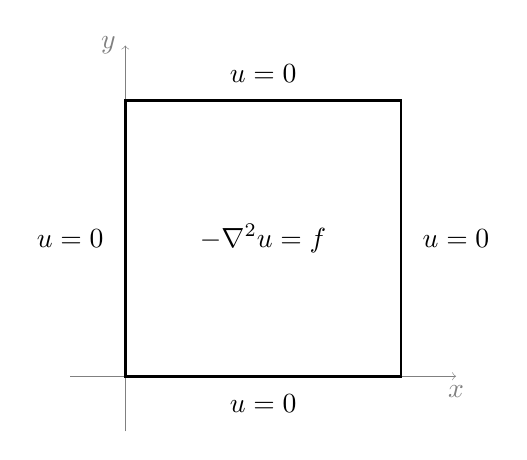
\begin{tikzpicture}[scale=3.5]
  \draw[->,gray,very thin] (-0.2,0.0) -- (1.2,0.0) node[below] {$x$};
  \draw[->,gray,very thin] (0.0,-0.2) -- (0.0,1.2) node[left] {$y$};
  \draw[line width=1.0pt] (0.0,0.0) -- (0.0,1.0) -- (1.0,1.0) -- (1.0,0.0) -- cycle;
  \node at (0.5,0.5) {$- \grad^2 u = f$};
  \node at (0.5,-0.1) {$u = 0$};
  \node at (0.5,1.1) {$u = 0$};
  \node at (-0.2,0.5) {$u = 0$};
  \node at (1.2,0.5) {$u = 0$};
\end{tikzpicture}
\caption{Our first, simple goal is to solve the Poisson equation on the unit square $\mathcal{S}$, with homogeneous Dirichlet boundary conditions.}
\label{fig:unitsquare}
\end{marginfigure}
\begin{align}
- \grad^2 u &= f \quad \text{ on } \mathcal{S}, \label{poissonsquare} \\
u &= 0 \quad \text{ on } \partial \mathcal{S}. \notag
\end{align}
The boundary of the unit square, denoted ``$\partial\mathcal{S}$'', is simply the union of four (closed) line segments.  The boundary conditions $u=0$ are called ``\emph{homogeneous Dirichlet}.''

The Poisson problem can model the electrostatic potential, the equilibrium distribution from certain random walks, the distribution of temperature in a conducting object at steady state, and many other other physical phenomena.  For example, in the context of heat conduction Fourier's law says $\bq = -k \grad u$, where $k$ is approximately constant if the variation in $u$ is not too large.  Conservation of energy for a solid says $c\rho \partial u/\partial t = - \Div\bq + f$ if $f$ describes a heat source within the domain.  At steady state these facts combine to give $0 = k \grad^2 u + f$, that is, Poisson's equation \eqref{poissonsquare}.  Holding the temperature fixed at zero along the boundary completes the problem.

For this chapter we will suppose that $f(x,y)$ is continuous and bounded on $\mathcal{S}$, so that we can compute its pointwise values.  With our homogeneous Dirichlet boundary conditions, and the assumptions on $f$, standard theory says that $u(x,y)$ exists and is continuous on the closed square $\overline{\mathcal{S}}$ \citep[Theorem 6 in section 5.6]{Evans}.\sidenote{A classical approach to showing existence starts by solving problem \eqref{poissonsquare} by Fourier series.  If $f$ is square-integrable then the coefficients $\hat f$ are square-integrable (Parseval's equality).  Because the Laplacian is elliptic and second-order, the coefficients $\hat u$ are square-integrable even when multiplied by the frequency squared.  By Cauchy-Schwarz, the Fourier series for $u$ is the limit of a sequence of continuous functions on $\overline{\mathcal{S}}$ which converge uniformly, so $u\in C^0(\overline{\mathcal{S}})$.}  Thus there is no ambiguity in the boundary condition ``$u=0$ on $\partial \mathcal{S}$,'' and also we can sensibly discuss the pointwise values $u(x,y)$.

Without any boundary conditions, the Poisson equation $-\grad^2 u = f$ alone is not a well-posed problem because if $u$ is a solution then $v=u+C$ is also a solution for any constant $C$.  (In fact there are constant solutions $w=C$ and many, many more to the Laplace equation $-\grad^2 w = 0$ on $\mathcal{S}$.)  However, with the Dirichlet boundary conditions in \eqref{poissonsquare}, the solution is unique if it exists \citep[Theorem 5 in section 2.2]{Evans}; \citep[subsection 5.2.1]{Ockendonetal2003}.


\section{A finite difference method: build the grid}

Because \eqref{poissonsquare} is a linear problem, finite-dimensional approximations of it are simply linear systems.  The finite-dimensional approximation in this Chapter comes from applying a \emph{finite difference} (FD) method.  In Chapter 3 we will apply a finite element approach instead.

\begin{marginfigure}
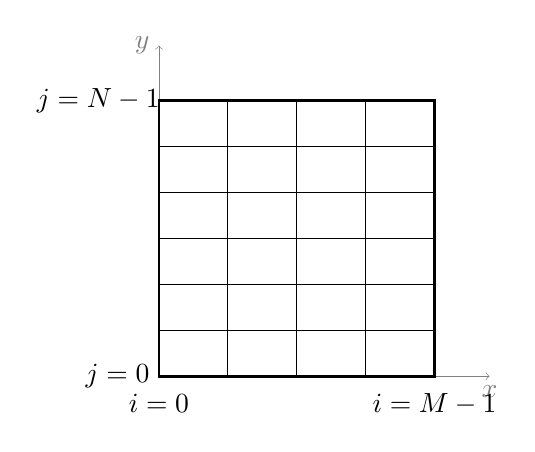
\begin{tikzpicture}[scale=3.5]
  \draw[->,gray,very thin] (0.0,0.0) -- (1.2,0.0) node[below] {$x$};
  \draw[->,gray,very thin] (0.0,0.0) -- (0.0,1.2) node[left] {$y$};
  \draw[line width=1.0pt] (0.0,0.0) -- (0.0,1.0) -- (1.0,1.0) -- (1.0,0.0) -- cycle;
  \node at (0.0,-0.1) {$i=0$};
  \node at (1.0,-0.1) {$i=M-1$};
  \node at (-0.15,0.0) {$j=0$};
  \node at (-0.22,1.0) {$j=N-1$};
  \pgfmathsetmacro\fourth{1.0/4.0}
  \pgfmathsetmacro\sixth{1.0/6.0}
  \draw[xstep=\fourth,ystep=\sixth,black,thin] (0.0,0.0) grid (1.0,1.0);
\end{tikzpicture}
\caption{A grid on the unit square $\mathcal{S}$, with $M=5$ and $N=7$.}
\label{fig:unitsquaregrid}
\end{marginfigure}

To start our FD method we put a \emph{structured grid} of $MN$ points on the unit square, as in Figure \ref{fig:unitsquaregrid}, with spacing $h_x=1/(M-1)$ and $h_y=1/(N-1)$ in the two directions.  The grid locations are $x_i = i\, h_x$ for $i = 0,1,\dots,M-1$ and $y_j = j\, h_y$ and $j=0,1,\dots,N-1$.

The construction of such a two-dimensional (2D) grid, and the distribution of it across processors, will be our first new idea from \PETSc, beyond the basics in Chapter 1.  Consider the lines of code in Figure \ref{code:dmdacreatetwod}.  They create a \PETSc \pDM object\sidenote{``\pDM'' might stand for ``data management'', but perhaps ``distributed mesh'' is better.} for a grid like Figure \ref{fig:unitsquaregrid}.

\clearpage
\cinputraw{dmdacreate2d.frag}{extract from c2poisson.c}{An example of creating a 2D \pDMDA.}{}{//START}{//STOP}{code:dmdacreatetwod}

A \pDM is an abstract type for describing the topology (i.e.~connectedness) of a grid, \emph{and} the way it is distributed across \MPI processes, \emph{and} the way each process can access data from its neighbors.  The specific variable \texttt{da} in Figure \ref{code:dmdacreatetwod} has type ``\pDMDA'', which is the subclass of \pDM s which are structured grids.

The Figure \ref{code:dmdacreatetwod} code will appear in \texttt{c2poisson.c} below, which solves Poisson's problem.  For now, if we do
\begin{Verbatim}[fontsize=\small]
  make c2poisson
  mpiexec -n 4 ./c2poisson -da_grid_x 5 -da_grid_y 7
\end{Verbatim}
then a structured grid will be distributed across the four processes exactly as in Figure \ref{fig:unitsquaregridparallel}.  Neither $M=5$ nor $N=7$ is divisible by two in this case, but \PETSc distributes the four ranks across the $MN=35$ nodes (grid points) as uniformly as possible given that each processor owns a rectangular subgrid.  In fact, the rank $0$ process has the most nodes (12) and rank $3$ has the least (6), so the load is only uniform within a factor of two, but larger grids will be better load-balanced.  \PETSc does the best it can.

\begin{marginfigure}
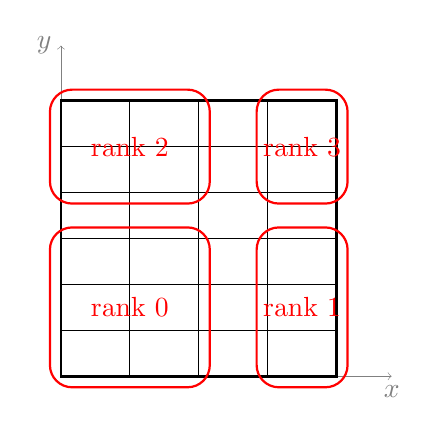
\begin{tikzpicture}[scale=3.5]
  \draw[->,gray,very thin] (0.0,0.0) -- (1.2,0.0) node[below] {$x$};
  \draw[->,gray,very thin] (0.0,0.0) -- (0.0,1.2) node[left] {$y$};
  \draw[line width=1.0pt] (0.0,0.0) -- (0.0,1.0) -- (1.0,1.0) -- (1.0,0.0) -- cycle;
  \pgfmathsetmacro\fourth{1.0/4.0}
  \pgfmathsetmacro\sixth{1.0/6.0}
  \draw[xstep=\fourth,ystep=\sixth,black,thin] (0.0,0.0) grid (1.0,1.0);
  \pgfmathsetmacro\dd{0.04}
  \pgfmathsetmacro\od{1.04}
  \pgfmathsetmacro\xap{2*\fourth + 0.04}
  \pgfmathsetmacro\xbm{3*\fourth - 0.04}
  \pgfmathsetmacro\yap{3*\sixth + 0.04}
  \pgfmathsetmacro\ybm{4*\sixth - 0.04}
  \pgfmathsetmacro\xamid{1*\fourth}
  \pgfmathsetmacro\xbmid{3.5*\fourth}
  \pgfmathsetmacro\yamid{1.5*\sixth}
  \pgfmathsetmacro\ybmid{5*\sixth}
  \draw[thick,rounded corners=8pt,color=red]
    (-\dd,-\dd) -- (-\dd,\yap) -- (\xap,\yap) -- (\xap,-\dd) -- cycle;
  \node[color=red] at (\xamid,\yamid) {rank $0$};
  \draw[thick,rounded corners=8pt,color=red]
    (\xbm,-\dd) -- (\od,-\dd) -- (\od,\yap) -- (\xbm,\yap) -- cycle;
  \node[color=red] at (\xbmid,\yamid) {rank $1$};
  \draw[thick,rounded corners=8pt,color=red]
    (-\dd,\ybm) -- (\xap,\ybm) -- (\xap,\od) -- (-\dd,\od) -- cycle;
  \node[color=red] at (\xamid,\ybmid) {rank $2$};
  \draw[thick,rounded corners=8pt,color=red]
    (\xbm,\ybm) -- (\od,\ybm) -- (\od,\od) -- (\xbm,\od) -- cycle;
  \node[color=red] at (\xbmid,\ybmid) {rank $3$};
\end{tikzpicture}
\caption{The same grid as in Figure \ref{fig:unitsquaregrid}, distributed across four \MPI processes (i.e.~with \texttt{rank} $\in \{0,1,2,3\}$) automatically by \texttt{DMDACreate2d()}.}
\label{fig:unitsquaregridparallel}
\end{marginfigure}

The fifth and sixth arguments ``\texttt{-10}'' to \texttt{DMDACreate2d()} in Figure \ref{code:dmdacreatetwod} are used to set default dimensions $M=10$ and $N=10$.  We have seen that these defaults are overridden by runtime options \texttt{-da\_grid\_x} and \texttt{-da\_grid\_y}.  However, if we do this,
 \begin{Verbatim}[fontsize=\small]
  mpiexec -n 4 ./c2poisson
\end{Verbatim}
then a structured grid will be distributed across the four processes as in Figure \ref{fig:unitsquaregrideight}, with each rank owning 25 nodes.  \PETSc itself can show the parallel layout by calling
\begin{Verbatim}[fontsize=\small]
  mpiexec -n 4 ./c2poisson -dm_view
\end{Verbatim}
or
\begin{Verbatim}[fontsize=\small]
  mpiexec -n 4 ./c2poisson -dm_view draw -draw_pause 2
\end{Verbatim}
The latter version shows the grid graphically, for two seconds.

\begin{marginfigure}
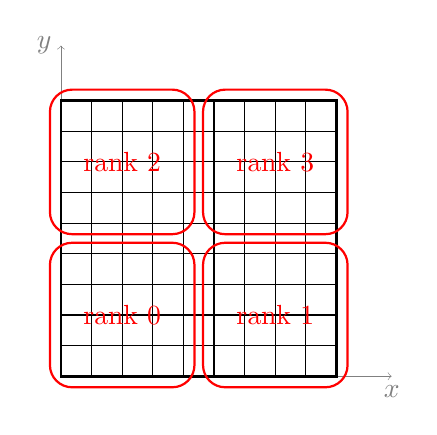
\begin{tikzpicture}[scale=3.5]
  \draw[->,gray,very thin] (0.0,0.0) -- (1.2,0.0) node[below] {$x$};
  \draw[->,gray,very thin] (0.0,0.0) -- (0.0,1.2) node[left] {$y$};
  \draw[line width=1.0pt] (0.0,0.0) -- (0.0,1.0) -- (1.0,1.0) -- (1.0,0.0) -- cycle;
  \pgfmathsetmacro\ninth{1.0/9.0}
  \draw[xstep=\ninth,ystep=\ninth,black,thin] (0.0,0.0) grid (1.0,1.0);
  \pgfmathsetmacro\dd{0.04}
  \pgfmathsetmacro\od{1.04}
  \pgfmathsetmacro\ap{4*\ninth + 0.04}
  \pgfmathsetmacro\bm{5*\ninth - 0.04}
  \pgfmathsetmacro\amid{2*\ninth}
  \pgfmathsetmacro\bmid{7*\ninth}
  \draw[thick,rounded corners=8pt,color=red]
    (-\dd,-\dd) -- (-\dd,\ap) -- (\ap,\ap) -- (\ap,-\dd) -- cycle;
  \node[color=red] at (\amid,\amid) {rank $0$};
  \draw[thick,rounded corners=8pt,color=red]
    (\bm,-\dd) -- (\od,-\dd) -- (\od,\ap) -- (\bm,\ap) -- cycle;
  \node[color=red] at (\bmid,\amid) {rank $1$};
  \draw[thick,rounded corners=8pt,color=red]
    (-\dd,\bm) -- (\ap,\bm) -- (\ap,\od) -- (-\dd,\od) -- cycle;
  \node[color=red] at (\amid,\bmid) {rank $2$};
  \draw[thick,rounded corners=8pt,color=red]
    (\bm,\bm) -- (\od,\bm) -- (\od,\od) -- (\bm,\od) -- cycle;
  \node[color=red] at (\bmid,\bmid) {rank $3$};
\end{tikzpicture}
\caption{An $M=10$ by $N=10$ grid distributed by \texttt{DMDACreate2d()} across four \MPI processes.}
\label{fig:unitsquaregrideight}
\end{marginfigure}

To explain the other options to \texttt{DMDACreate2d()} used in Figure \ref{code:dmdacreatetwod}, we quote the \PETSc manual pages description of that method:

\clearpage
\noindent\hrulefill
\begin{Verbatim}[fontsize=\small]
DMDACreate2d(MPI_Comm comm, DMBoundaryType bx, DMBoundaryType by,
  DMDAStencilType stype, PetscInt M, PetscInt N, PetscInt m, PetscInt n,
  PetscInt dof, PetscInt s, const PetscInt lx[], const PetscInt ly[],
  DM *da)
\end{Verbatim}
where
\small
\begin{itemize}[align=left]
\item[\texttt{comm}]   MPI communicator \\
\item[\texttt{bx,by}]  type of ghost nodes the array have; use one of \texttt{DM\_BOUNDARY\_NONE, DM\_BOUNDARY\_GHOSTED, DM\_BOUNDARY\_PERIODIC} \\
\item[\texttt{stype}] stencil type; use either \texttt{DMDA\_STENCIL\_BOX} or \texttt{DMDA\_STENCIL\_STAR} \\
\item[\texttt{M,N}]	   global dimension in each direction of the array; use \texttt{-M} and or \texttt{-N} to indicate that it may be set to a different value from the command line with \texttt{-da\_grid\_x <M> -da\_grid\_y <N>} \\
\item[\texttt{m,n}]   corresponding number of processors in each dimension (or \texttt{PETSC\_DECIDE} to have calculated) \\
\item[\texttt{dof}]     number of degrees of freedom per node \\
\item[\texttt{s}]       stencil width \\
\item[\texttt{lx,ly}]  arrays containing the number of nodes in each cell along the x and y coordinates, or \texttt{NULL}; if non-null, these must be of length as m and n, and the corresponding m and n cannot be \texttt{PETSC\_DECIDE}; the sum of the \texttt{lx[]} entries must be M, and the sum of the \texttt{ly[]} entries must be N \\
\item[\texttt{da}]      output: the resulting distributed array object 
\end{itemize}
\normalsize
\noindent\hrulefill
\medskip

In Figure \ref{code:dmdacreatetwod}, the first argument is a serial or parallel \MPI communicator.  In the second and third arguments we have used ``\texttt{DM\_BOUNDARY\_NONE}'' because our Dirichlet boundary condition does not require communication to the next process' domain, nor periodic wrapping.  In the fourth argument we use \texttt{DMDA\_STENCIL\_STAR} because only cardinal neighbors of a grid point are used when forming the matrix; we will address the FD ``stencil'' below.  As already noted, the fifth and sixth arguments set $M=10,N=10$ as override-able grid defaults.  In the next two arguments we indeed use ``\texttt{PETSC\_DECIDE}'' to have \PETSc parallel-decompose our grid according to the size of (i.e.~number of processes in) the \MPI communicator.  The next two arguments, in the ninth and tenth positions, say that our PDE is scalar (\texttt{dof}$=1$) and that the FD method only needs one neighbor in each direction (\texttt{s}$=1$).  The next two arguments are \texttt{NULL} because we are \emph{not} telling \PETSc how to distribute processes over the grid; it \texttt{DECIDE}s for itself.  Finally, the \pDMDA object is created as an output.

The call to \texttt{DMDASetUniformCoordinates()} in Figure \ref{code:dmdacreatetwod} sets the domain to be $[0,1]\times[0,1]$.  The last two arguments are ignored in this case but would set limits on the third dimension in 3D.

To wrap up our coverage of creating grids, the standard \PETSc view of what \pDM s ``look like'' is in Figure \ref{fig:petscghostvalues}.  On the left is a version of what we have done in the code in Figure \ref{code:dmdacreatetwod}, namely create a structured grid \pDM.  The one shown in Figure \ref{fig:petscghostvalues} has \texttt{DMDA\_STENCIL\_BOX} stencil type, unlike ours.  On the right is an unstructured grid, of the type created in Chapter 3 for the finite element method.  In both cases the figure shows nodes owned by a given process (red ``local'' nodes) and those other nodes that are accessible by the local process (blue ``ghost'' nodes).  We will see such local/ghost node types in all examples in this book.

\begin{figure}
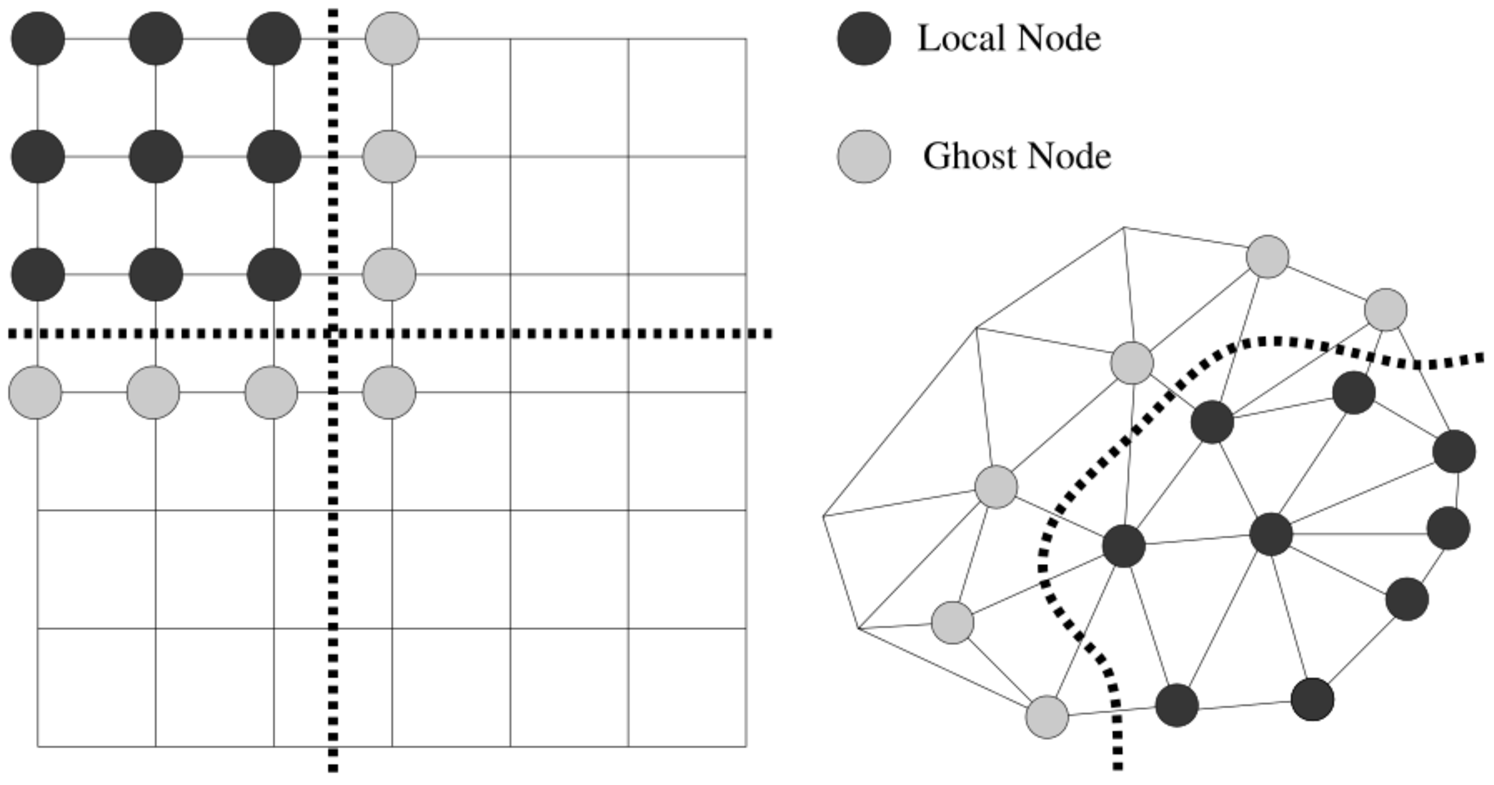
\includegraphics[width=\textwidth]{petscghostvalues}
\caption{\PETSc's parallel decomposition of structured and unstructured grids, showing owned (``local'') and accessible (``ghost'') nodes for one process.}
\label{fig:petscghostvalues}
\end{figure}


\section{A finite difference method: assemble the linear system}

Recall we were trying to approximate PDE problem \eqref{poissonsquare}.  Having built a structured grid we can now return to the FD method.

By a well-known Taylor's theorem argument \citep{MortonMayers}, for any function $F(x)$ which is sufficiently smooth, we have
    $$F''(x) = \frac{F(x+h) - 2 F(x) + F(x-h)}{h^2} + O(h^2)$$
as $h$ goes to zero.  This formula, applied to partial derivatives, will give an approximation of the Laplacian in problem \eqref{poissonsquare}.

Let $U_{i,j}$ be the gridded approximation to the exact value $u(x_i,y_j)$ of the solution $u$,\sidenote{This is an important sentence!  We \emph{compute} values $U_{i,j}$ from the finite difference equations.  We generally \emph{don't know} the values of the exact solution on the grid, namely $u(x_i,y_j)$.  Of course we want the former to be close to the latter.}  and also denote $f_{i,j} = f(x_i,y_j)$.  Then we have this FD approximation to problem \eqref{poissonsquare}:
\begin{equation}
- \frac{U_{i+1,j} - 2 U_{i,j} + U_{i-1,j}}{h_x^2} - \frac{U_{i,j+1} - 2 U_{i,j} + U_{i,j-1}}{h_y^2} = f_{i,j}. \label{poissonsquareFDearly}
\end{equation}
Equation \eqref{poissonsquareFDearly} applies for all of the interior points where $1 \le i \le M-2$ and $1 \le j \le N-2$.  The boundary conditions in \eqref{poissonsquare} become
\begin{equation}
U_{0,j} = 0, \quad U_{M-1,j} = 0, \quad U_{i,0} = 0, \quad U_{i,N-1} = 0, \label{poissonsquareFDbcs}
\end{equation}
for all $i,j$.

At location $(x_i,y_j)$, equation \eqref{poissonsquareFDearly} relates the unknown $U_{i,j}$ to its four cardinal neighbors $U_{i+1,j}$, $U_{i-1,j}$, $U_{i,j+1}$, and $U_{i,j-1}$.  This pattern is a \emph{stencil}, in particular a ``star'' stencil, as shown in Figure \ref{fig:unitsquaregridstencil}.  A ``box'' stencil would also involve all the diagonal neighbors, so an equation using a star stencil relates at most five unknowns in 2D, while one with a box stencil relates at most nine unknowns in 2D.

\begin{marginfigure}
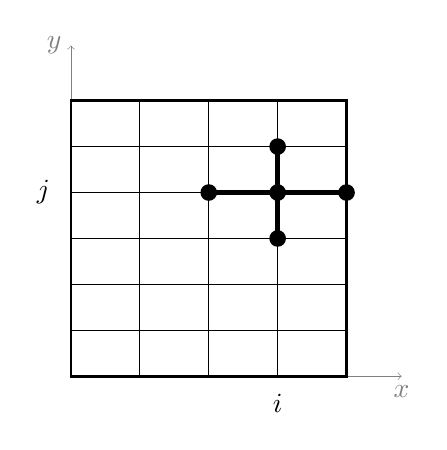
\begin{tikzpicture}[scale=3.5]
  \draw[->,gray,very thin] (0.0,0.0) -- (1.2,0.0) node[below] {$x$};
  \draw[->,gray,very thin] (0.0,0.0) -- (0.0,1.2) node[left] {$y$};
  \draw[line width=1.0pt] (0.0,0.0) -- (0.0,1.0) -- (1.0,1.0) -- (1.0,0.0) -- cycle;
  \node at (0.75,-0.1) {$i$};
  \node at (-0.1,0.666667) {$j$};
  \filldraw (0.50,0.666667) circle (0.8pt);
  \filldraw (0.75,0.666667) circle (0.8pt);
  \filldraw (1.00,0.666667) circle (0.8pt);
  \filldraw (0.75,0.5) circle (0.8pt);
  \filldraw (0.75,0.833333) circle (0.8pt);
  \draw[line width=2.0pt] (0.50,0.666667) -- (1.00,0.666667);
  \draw[line width=2.0pt] (0.75,0.5)  -- (0.75,0.833333);
  \draw[xstep=0.25,ystep=0.166667,black,thin] (0.0,0.0) grid (1.0,1.0);
\end{tikzpicture}
\caption{A ``star'' stencil, shown on the same grid as in Figure \ref{fig:unitsquaregrid}, at $i=3$ and $j=4$.}
\label{fig:unitsquaregridstencil}
\end{marginfigure}

Equations \eqref{poissonsquareFDearly} and \eqref{poissonsquareFDbcs} form a linear system of $K=MN$ equations in which we choose to treat all $K$ locations on the grid as unknowns.  To shown this linear system in traditional form
\begin{equation}
A \bu = \bb,
\end{equation}
where $A$ is a $K\times K$ matrix and $\bu,\bb$ are $K\times 1$ column vectors, we must order the unknowns.  This ordering will be used internally by \PETSc in a code that uses a \pDMDA, and we use it here for displaying the system, but the code we will actually write uses the grid-wise coordinates $(i,j)$.  One could write this ordering as
\begin{equation}
    U_k = U_{i,j} \quad \text{ where } \quad k = j\,M + i. \label{orderingfd}
\end{equation}
We will let \PETSc do such index transformations internally, because, as we will see, it has tools for $i,j$-type indexing.  Now is a good time to show the linear system itself, and the ordering, in a small case.

\begin{marginfigure}
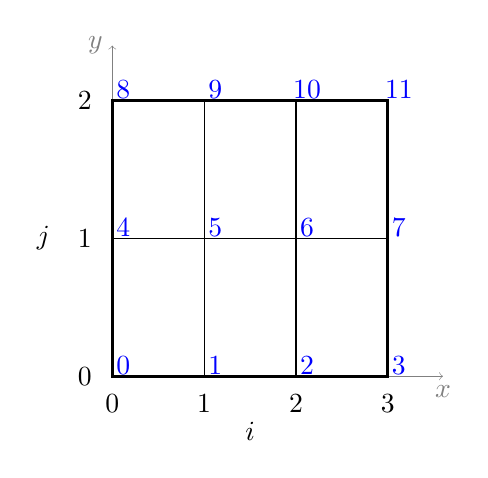
\begin{tikzpicture}[scale=3.5]
  \draw[->,gray,very thin] (0.0,0.0) -- (1.2,0.0) node[below] {$x$};
  \draw[->,gray,very thin] (0.0,0.0) -- (0.0,1.2) node[left] {$y$};
  \draw[line width=1.0pt] (0.0,0.0) -- (0.0,1.0) -- (1.0,1.0) -- (1.0,0.0) -- cycle;
  \pgfmathsetmacro\third{1.0/3.0}
  \pgfmathsetmacro\half{1.0/2.0}
  \node at (0.0,-0.1) {$0$};
  \node at (\third,-0.1) {$1$};
  \node at (\half,-0.2) {$i$};
  \node at (2*\third,-0.1) {$2$};
  \node at (1.0,-0.1) {$3$};
  \node at (-0.1,0.0) {$0$};
  \node at (-0.1,0.5) {$1$};
  \node at (-0.25,0.5) {$j$};
  \node at (-0.1,1.0) {$2$};
  \draw[xstep=\third,ystep=\half,black,thin] (0.0,0.0) grid (1.0,1.0);
  \pgfmathsetmacro\dd{0.04}
  \foreach \y in {0,1,2}
    \foreach \x in {0,1,2,3} {
      \pgfmathsetmacro\k{4*\y+\x}
      \draw[color=blue] (\x*\third+\dd,\y*\half+\dd) node{\pgfmathprintnumber[fixed]{\k}};
    }
\end{tikzpicture}
\caption{Ordering of unknowns \eqref{orderingfd} on a $M=4$ and $N=3$ grid.  Index $k = j\,M + i$ is shown in {\color{blue} blue}.}
\label{fig:unitsquaregridordering}
\end{marginfigure}

\medskip\noindent\hrulefill
\begin{example} In the $M=4$ and $N=3$ case we have the grid and variable ordering shown in Figure \ref{fig:unitsquaregridordering}.  Note $h_x=1/3$ and $h_y=1/2$.  Equations \eqref{poissonsquareFDearly} and \eqref{poissonsquareFDbcs} are an invertible system of $K=12$ equations.  Only the $k=5$ and $k=6$ equations are not boundary conditions \eqref{poissonsquareFDbcs}:
\setcounter{MaxMatrixCols}{20}
\begin{equation*}
\begin{bmatrix}
1 &  &  &  &  &  &  &  &  &  &  &  \\
  & 1&  &  &  &  &  &  &  &  &  &  \\
  &  & 1&  &  &  &  &  &  &  &  &  \\
  &  &  & 1&  &  &  &  &  &  &  &  \\
  &  &  &  & 1&  &  &  &  &  &  &  \\
  & c&  &  & b& a& b&  &  & c&  &  \\
  &  & c&  &  & b& a& b&  &  & c&  \\
  &  &  &  &  &  &  & 1&  &  &  &  \\
  &  &  &  &  &  &  &  & 1&  &  &  \\
  &  &  &  &  &  &  &  &  & 1&  &  \\
  &  &  &  &  &  &  &  &  &  & 1&  \\
  &  &  &  &  &  &  &  &  &  &  & 1
\end{bmatrix}
\begin{bmatrix}
U_{0,0} \\
U_{1,0} \\
U_{2,0} \\
U_{3,0} \\
U_{0,1} \\
U_{1,1} \\
U_{2,1} \\
U_{3,1} \\
U_{0,2} \\
U_{1,2} \\
U_{2,2} \\
U_{3,2}
\end{bmatrix}
=
\begin{bmatrix}
0 \\
0 \\
0 \\
0 \\
0 \\
f_{1,1} \\
f_{2,1} \\
0 \\
0 \\
0 \\
0 \\
0
\end{bmatrix}
\end{equation*}
where $a = 2/h_x^2 + 2/h_y^2 = 26$, $b = - 1/h_x^2 = -9$ and $c = - 1/h_y^2 = -4$.

Note that the matrix $A$ is not symmetric, and it is not well-scaled for such a small example.  For instance, its 2-norm condition number \citep{TrefethenBau} is $\cond(A) = \|A\|_2 \|A^{-1}\|_2 = 43.16$.
\end{example}
\noindent\hrulefill

Before assembling the system, by writing \PETSc code, there are two nontrivial observations about it.  First, the equations \eqref{poissonsquareFDearly} have very different ``scaling'' from those in \eqref{poissonsquareFDbcs}.  For example, if $M=N=1001$, so that $h_x=h_y=0.001$, then the coefficient of $U_{i,j}$ in \eqref{poissonsquareFDearly} is $4/(.001)^2 = 4 \times 10^6$, where as the coefficients of $U_{i,j}$ along the boundary in \eqref{poissonsquareFDbcs} are equal to 1.  Therefore we multiply equation \eqref{poissonsquareFDearly} by the grid cell area $h_x h_y$ to get
\begin{align}
&\left(2 \frac{h_y}{h_x} + 2 \frac{h_x}{h_y}\right) U_{i,j} - \frac{h_y}{h_x}\left(U_{i+1,j} + U_{i-1,j}\right)  - \frac{h_x}{h_y}\left(U_{i,j+1} + U_{i,j-1}\right) \label{poissonsquareFD} \\
&\qquad = h_x h_y f_{i,j}. \notag
\end{align}
Using \eqref{poissonsquareFD}, as long as the cell aspect ratio $\max\{h_y/h_x,h_x/h_y\}$ is not too large, all the equations in the system, including the boundary conditions, will have coefficients of comparable size.  Note that if $h_x=h_y$ then the diagonal entries are equal to $4$ and the off-diagonal entries are $-1$.

Second, our equations can be interpreted to give a \emph{symmetric} matrix $A$.  This opens up a larger range of linear algebra methods for solving the system efficiently.  For example, in the $i=1$ case of \eqref{poissonsquareFD}, i.e.~at a grid point adjacent to the left-hand boundary of the square, the boundary location value $U_{0,j}$ appears in the equation.  The matrix in the linear system will be symmetric if we systematically ``move'' such values to the right-hand side as known (and zero) instead of inserting a ``$1$'' into the corresponding matrix locations.  That is, we make off-diagonal zero entries in the columns corresponding to known boundary values, in addition to the off-diagonal zeros in rows corresponding to known boundary values.  With these two modifications we can redo the above $M=4$ and $n=3$ example.

\medskip\noindent\hrulefill
\begin{example} For the same $M=4$ and $N=3$ case shown in Figure \ref{fig:unitsquaregridordering}, equations \eqref{poissonsquareFDbcs} and \eqref{poissonsquareFD} become
\begin{equation*}
\begin{bmatrix}
1 &  &  &  &  &  &  &  &  &  &  &  \\
  & 1&  &  &  &  &  &  &  &  &  &  \\
  &  & 1&  &  &  &  &  &  &  &  &  \\
  &  &  & 1&  &  &  &  &  &  &  &  \\
  &  &  &  & 1&  &  &  &  &  &  &  \\
  &  &  &  &  & \alpha& \beta&  &  &  &  &  \\
  &  &  &  &  & \beta& \alpha&  &  &  &  &  \\
  &  &  &  &  &  &  & 1&  &  &  &  \\
  &  &  &  &  &  &  &  & 1&  &  &  \\
  &  &  &  &  &  &  &  &  & 1&  &  \\
  &  &  &  &  &  &  &  &  &  & 1&  \\
  &  &  &  &  &  &  &  &  &  &  & 1
\end{bmatrix}
\begin{bmatrix}
U_{0,0} \\
U_{1,0} \\
U_{2,0} \\
U_{3,0} \\
U_{0,1} \\
U_{1,1} \\
U_{2,1} \\
U_{3,1} \\
U_{0,2} \\
U_{1,2} \\
U_{2,2} \\
U_{3,2}
\end{bmatrix}
=
\begin{bmatrix}
0 \\
0 \\
0 \\
0 \\
0 \\
(1/6) f_{1,1} \\
(1/6) f_{2,1} \\
0 \\
0 \\
0 \\
0 \\
0
\end{bmatrix}
\end{equation*}
where $\alpha = 2 (h_y/h_x) + 2 (h_x/h_y) = 13/3$ and $\beta = - h_y/h_x = 3/2$.  The matrix is better-scaled, with $\cond(A)=5.83$.
\end{example}
\noindent\hrulefill


FIXME: explain Mat assembly tools, including DALocalInfo and MatStencil

\clearpage

\cinput{structuredlaplacian.c}{Fill matrix entries using \texttt{MatSetValuesStencil}.}{//CREATEMATRIX}{//ENDCREATEMATRIX}{code:structuredlaplacian}

\cinputpart{c2poisson.c}{The right side of equation \eqref{poissonsquareFD} comes from differentiating the exact solution, which this method also computes.}{I}{//RHS}{//ENDRHS}{code:ctwopoissonrhs}

\cinputpart{c2poisson.c}{Set up \pDMDA \texttt{da} and \pMat \texttt{A} objects, and assemble the latter by calling \texttt{formlaplacian()}.}{II}{//CREATE}{//ENDCREATE}{code:ctwopoissoncreate}

\cinputpart{c2poisson.c}{Solve using \pKSP, and report on solution.}{III}{//SOLVE}{//ENDSOLVE}{code:ctwopoissonsolve}

\section{Runtime control of linear solver}

FIXME: basic Krylov theory

\section{Time-dependent heat equation}

FIXME: we WON'T do explicit, but it would look like ...

FIXME: use TS for backward-euler
 % chapter 2


This Chapter returns to the Poisson equation in two dimensions.  We implement a finite element method (FEM) for an unstructured triangular mesh which covers a general polygonal domain.  Our code solves certain nonlinear generalizations of the standard linear problem, but these are different nonlinear forms from the $p$-Laplacian problem in the previous Chapter.

Our approach is to
\begin{center}
\emph{first do element-wise assembly of the residual equations,}
\end{center}
and thereby get a functioning \pSNES-based code.  We will not even think about matrices as we write the initial code.  Only after making sure it works do we
\begin{center}
\emph{then write additional code to assemble an approximate Jacobian matrix.}
\end{center}

We do the following new tasks:
\begin{itemize}
\item implement Neumann boundary conditions,
\item read a triangular mesh from a file into \PETSc \pVecs and \pISs,
\item index that mesh unstructured way, and
\item pre-allocate a \PETSc \pMat.
\end{itemize}

The example here contrasts with the rectangular-element ($Q^1$) FEM of the last Chapter in that it does not use a \pDMDA.  That type is limited to structured-grid topology.  Instead we implement a minimal, and naive, mesh-topology infrastructure, which substantially increases our workload.  The relatively-simple \Triangle program generates ASCII files describing the mesh.  An ``index set'' \pIS  type holds the global indices of nodes and triangles (elements).  \pVec and \pMat objects, used for the solution and Jacobian respectively, are indexed through the \pIS values.  Thus the benefits of \PETSc's mesh-topology \pDM tools, including \pDMDA in previous Chapters and \pDMPlex in Chapter \ref{chap:dp}, become clearer by forgoing them here.

In contrast with earlier and latter Chapters, we generate a code that only works on one MPI process (i.e.~a serial code).  At the end of the Chapter briefly consider the additional constructs needed to distribute a mesh across many processes.  Instead of even attempting an \emph{ad hoc} approach, however, these considerations motivate the \pDMPlex example in Chapter \ref{chap:dp}.

The residual equations $\bF(\bu)=0$, the nonlinear system seen by the \pSNES solver, is the discretized weak form of the PDE.  Our direct construction of these equations roughly follows the residual implementations of Chapters \ref{chap:nl}--\ref{chap:of}.  The FEM ``stiffness'' matrix $A$, and corresponding linear system $A\bx = \bb$, which is to say the major pieces of typical FEM introductions \citep{Braess2007,Elmanetal2005}, arise here as the Jacobian, and Newton step, respectively, when solving $\bF(\bu)=0$.  In our first runs, done before writing any matrix-assembly code, the \pSNES solver approximates this linear system through finite-differencing of evaluations of $\bF$.  Eventually we will only assemble a Jacobian which is accurate for the linear case.  For the smooth nonlinear case tested here, this inaccurate linearization suffices.


\section{A 2D nonlinear Poisson problem}

\begin{marginfigure}
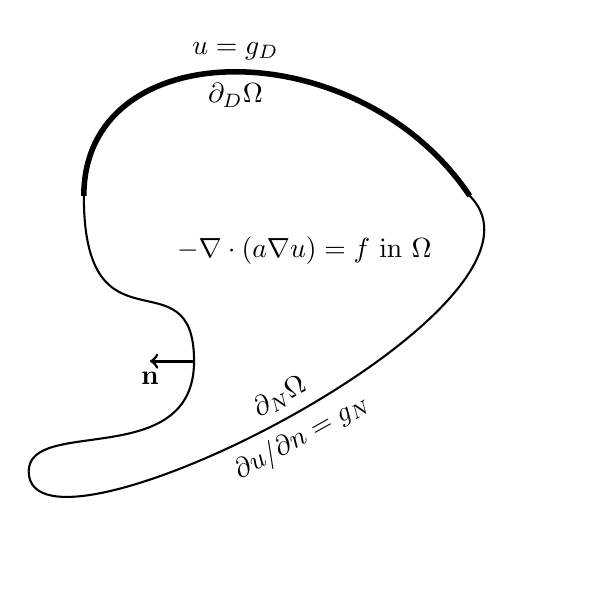
\begin{tikzpicture}[scale=0.7]
%\draw[gray,very thin] (-2,-6) grid (8,3);
\draw[line width=2pt] (0,0) .. controls (0,3) and (5,3) .. node[sloped,above] {$u=g_D$} node[sloped,below] {$\partial_D\Omega$} (7,0);
\draw[line width=0.75pt] (7,0) .. controls (9,-2) and (-1,-7) .. node[sloped,above] {$\partial_N\Omega$} node[sloped,below] {$\partial u/\partial n = g_N$} (-1,-5);
\draw[line width=0.75pt] (-1,-5) .. controls (-1,-4) and (2,-5) .. (2,-3);
\draw[line width=0.75pt] (2,-3) .. controls (2,-1) and (0,-3) .. (0,0);
\draw[->,line width=1.0pt] (2,-3) -- (1.2,-3) node[below] {$\bn$}; % normal vector
\draw (4,-1) node {$- \Div (a \grad u) = f$ in $\Omega$};
\end{tikzpicture}


\caption{Problem \eqref{eq:un:poissonstrong} on a domain.}
\label{fig:un:generalpoissondomain}
\end{marginfigure}

Let $\Omega \subset \RR^2$ be a bounded (open) region.  Suppose its boundary $\partial\Omega$ is well-behaved (polygonal or Lipschitz-continuous \citep[section 1.2]{Ciarlet2002}).  Suppose $\partial\Omega$ is decomposed into (measurable) disjoint subsets $\partial_D \Omega$ and $\partial_N \Omega$ whose union is the entire boundary $\partial \Omega$.

The Poisson problem in Chapter \ref{chap:st} is based on the equation $- \grad^2 u = f$.  We allow a more general nonlinear form here.  Let $a(x,y,u)$ and $f(x,y,u)$ be continuous functions, and assume there is $\eps>0$ so that
    $$a(x,y,u) \ge \eps > 0.$$
That is, we require \emph{uniform ellipticity} \citep{Evans2010}.  The strong form also includes boundary conditions, here nonhomogeneous Dirichlet and Neumann boundary conditions.  Thus the  nonlinear Poisson (diffusion) \emph{strong form} we solve is to find $u(x,y)$ so that
\begin{align}
- \Div \left(a(x,y,u) \grad u\right) &= f(x,y,u) \quad \text{ on } \Omega, \label{eq:un:poissonstrong} \\
u &= g_D \quad \text{ on } \partial_D \Omega, \notag \\
\frac{\partial u}{\partial n} &= g_N \quad \text{ on } \partial_N \Omega. \notag
\end{align}
By definition, $\partial u/\partial n = \bn \cdot \grad u$ where $\bn$ is the outward unit normal on $\partial \Omega$.

The data of problem \eqref{eq:un:poissonstrong}, besides the region $\Omega$ and its boundary, includes a \emph{diffusion coefficient} $a$, a \emph{source term} $f$, \emph{Dirichlet data} $g_D$, and \emph{Neumann data} $g_N$.  For the purpose of numerical solutions we will simply assume that the boundary data is continuous.  Poisson problem \eqref{poissonsquare} in Chapter \ref{chap:st} is the homogeneous Dirichlet case where $\Omega$ is the square, $a\equiv 1$, $f=f(x,y)$ is independent of the solution $u$, $\partial_D \Omega = \partial \Omega$, $\partial_N \Omega = \emptyset$, and $g_D=0$.

Problem \eqref{eq:un:poissonstrong} is not the most general (nonlinear) Poisson problem.  Specifically, one could allow more general \emph{Robin} boundary conditions $\alpha u + \beta \frac{\partial u}{\partial n} = \gamma$ where, generally, $\alpha,\beta,\gamma$ could vary along the boundary \citep{Elmanetal2005}.  One could also allow $a$ and/or $f$ to depend on the gradient of $u$, as does $a=|\grad u|^{p-2}$ in the $p$-Laplacian equation of Chapter \ref{chap:of}.

As \eqref{eq:un:poissonstrong} is stated there may be no solution where ``$\Div(a\grad u)$'' makes sense as a continuous function, even for polygonal regions and continuous data.  That is, there may be no $u\in C^2(\Omega) \cap C(\overline \Omega)$ so that $-\Div(a\grad u) = f$.  A solution exists, however, in the linear case at least, if we convert \eqref{eq:un:poissonstrong} to a \emph{weak form}.  A weak formulation arose in Chapter \ref{chap:of} as the gradient of an objective function, but the weak form here is generally not of that type.  We will derive it from the strong form in the traditional way, by multiplying by a test function and integrating.


\section{Weak form with general boundary values}

Recall $L^2(\Omega)$ is the space of square-integrable real functions on $\Omega$.  Define the following Sobolev space \citep{Evans2010}:
    $$H^1(\Omega) = \left\{u \,:\, u \in L^2(\Omega) \,\&\, \grad u \in L^2(\Omega)\right\}.$$
Definition \eqref{eq:of:sobolevdefn} of $W^{1,p}(\Omega)$ includes this space so that $H^1(\Omega) = W^{1,2}(\Omega)$.  This Chapter uses the notation with ``$H$'' standing for Hilbert.

We use two subsets of $H^1(\Omega)$: \emph{trial functions} come from $H_{g}^1(\Omega)$, which denotes the functions with value $g_D$ along $\partial_D \Omega$, and \emph{test functions} come from $H_{0}^1(\Omega)$, with value $0$ along $\partial_D \Omega$.  Note that $H_{0}^1(\Omega)$ is a linear subspace of $H^1(\Omega)$ while generally $H_{g}^1(\Omega)$ is not.

Now choose any $v\in H_{0}^1(\Omega)$, multiply the first equation in \eqref{eq:un:poissonstrong} by $v$, and integrate by parts:
\begin{equation*}
\int_\Omega a(u) \grad u \cdot \grad v - \int_{\partial\Omega} \frac{\partial u}{\partial n} v = \int_\Omega f(u) v.
\end{equation*}
(In writing such integrals we generally show dependence on the solution $u$ but suppress it for $x,y$ so that $a(x,y,u)=a(u)$, and similarly for $f$.)  Next we use the boundary information, namely that $v=0$ on $\partial_D\Omega$ and $\frac{\partial u}{\partial n}=g_N$ on $\partial_N\Omega$:
\begin{equation}
\int_\Omega a(u) \grad u \cdot \grad v = \int_\Omega f(u) v + \int_{\partial_N\Omega} g_N v\quad \text{ for any } v\in H_{0}^1(\Omega). \label{eq:un:poissonweak}
\end{equation}
Equation \eqref{eq:un:poissonweak} is the \emph{weak formulation} of \eqref{eq:un:poissonstrong}, and any $u \in H_{g}^1(\Omega)$ satisfying it is a \emph{weak solution}.  Observe that the Dirichlet boundary conditions $g_D$ are incorporated into defining $H_{g}^1(\Omega)$ while the Neumann boundary data $g_N$ appears in the weak form \eqref{eq:un:poissonweak}.

Summarizing the ``rules'' for passing between the strong \eqref{eq:un:poissonstrong} and weak \eqref{eq:un:poissonweak} formulations might clarify the situation:\begin{itemize}
\item A well-behaved function $u \in C^2(\Omega) \cap C(\overline \Omega)$ which satisfies the strong form also solves the weak form.  (The derivation above shows this.)
\item If $u \in H_{g}^1(\Omega)$ solves the weak form then we accept it, by definition, as a solution.   If it is also well-behaved (i.e.~$u \in C^2(\Omega) \cap C(\overline \Omega)$) then we may reverse the derivation to show it solves the strong form.  (Not shown, but see \citet{Evans2010}.)
\end{itemize}

Consider the linear case where functions $a$ and $f$ are independent of $u$.  If $\partial_D \Omega$ has positive measure then a solution to weak formulation \eqref{eq:un:poissonweak} exists and is unique (\emph{well-posedness}; \citep{Ciarlet2002,Evans2010}).  There exist conditions on the domain (e.g.~convex polygon) and the boundary data under which one can furthermore show that $u$ solving \eqref{eq:un:poissonweak} is in $C^2(\Omega) \cap C(\overline \Omega)$ (\emph{regularity}; \citep{Evans2010}).  Such theoretical matters are mostly beyond our scope.

In nonlinear cases each particular problem must be analyzed for well-posedness.  In terms of practical computation, particular nonlinear cases covered by our method, and solvable using our code, include 2D versions of
\begin{itemize}
\item the \emph{Bratu} equation\sidenote{Exercises \ref{chap:nl}.\ref{exer:nl:bratu} and \ref{chap:un}.\ref{exer:un:bratu} solve the 1D and 2D versions, respectively.} if $a\equiv 1$ and $f=\lambda e^u$, and
\item ``uniformized'' versions of the \emph{porous medium} equation \citep{Ockendonetal2003}, in which, for example, $a=u^{m-1}+\eps$ for some $m\ge 1$ and $\eps>0$.
\end{itemize}


\section{A $P^1$ FEM}

A FEM for the Poisson problem comes from requiring the weak formulation \eqref{eq:un:poissonweak} to be true for $u$ in a finite-dimensional subspace of $H_{g}^1(\Omega)$, and for test functions $v$ ranging over a basis of a finite-dimensional subspace of $H_{0}^1(\Omega)$.\sidenote{An FEM is \emph{conforming} if these subspace claims are accurate.  Otherwise one is guilty of \emph{variational crimes} \citep{Ciarlet2002} with \emph{nonconforming elements} \citep{Braess2007}.}  In the \emph{Galerkin} method here, these subspaces, built upon a triangulation of $\Omega$, will be nearly the same.

To make our test function space $H_{0}^1(\Omega)$ a true subspace of $H^1(\Omega)$ we require that $\Omega$ be polygonal, with $\partial\Omega$ a closed polygon (Figure \ref{fig:un:polygon}).  Furthermore we require that segments which form the polygon $\partial\Omega$ be either entirely in $\partial_D\Omega$ or entirely in $\partial_N\Omega$.

We will assume $\partial_D\Omega$ is a closed set.  Furthermore we assume it contains at least one segment of positive length.  As suggested above, this leads to well-posedness of the continuum problem, at least in the linear case.

\begin{marginfigure}
\input{tmp/blob.tikz}
\caption{A polygonal domain $\Omega$ with $\partial_D\Omega$ in bold.}
\label{fig:un:polygon}
\end{marginfigure}

By definition, a \emph{triangulation} is a finite set of non-overlapping, non-empty open triangles $\triangle_k\subset \RR^2$ which tile $\Omega$:
\begin{equation}
\Th = \left\{\triangle_k \,\Big|\, \cup_k \overline{\triangle}_k = \overline{\Omega} \, \text{ and} \,\, \Omega_k \cap \Omega_l = \emptyset \, \text{ if } k\ne l\right\}. \label{eq:un:triangulation}
\end{equation}
We index the $K$ triangles (elements) in $\Th$ by $k=0,\dots,K-1$.  The $N$ vertices (nodes) in $\Th$ are indexed by $j=0,1,\dots,N-1$, with locations
\begin{equation*}
\bx_j = (x_j,y_j).
\end{equation*}

An example triangulation $\Th$ is shown in Figure \ref{fig:un:number-mesh}.  The subscript ``$h$'' in ``$\Th$,'' traditional notation, denotes the typical or maximum size $h$ (e.g.~diameter) of the triangles.  It serves as a reminder of our desired limit $h\to 0$.  In contrast to many references--e.g.~\citet{Elmanetal2005}, which we follow in many ways---all numbering here is zero-based, suitable for a C implementation.

We will use $P^1$ finite elements \citep{Elmanetal2005} so that our test and trial functions are continuous and linear on each $\triangle_k$.  On each triangle $\triangle_k$, such functions have three degrees of freedom.  We make think of these as the coefficients in the linear formula $a + b x + c y$, but in fact there are better local bases than $\{1,x,y\}$; see below.

For each node $j$ there is a basis (``hat'') function  $\psi_j(x,y)$ which is linear on each triangle, continuous on all of $\overline{\Omega}$, and equal to one at only one node $j$,
\begin{equation*}
\psi_j(\bx_i) = \delta_{ij}.
\end{equation*}
See Figure \ref{fig:un:hatfunction}.  (Compare Figure \ref{fig:of:q1hat}.)  Functions $\psi_j$ are in $H^1(\Omega)$ \citep{Braess2007}, with piecewise-constant partial derivatives $\partial\psi_j/\partial x$ and $\partial\psi_j/\partial y$.  The set $\{\psi_j\}_{j=0,\dots,N-1}$ is linearly-independent.

\begin{marginfigure}
\input{tmp/blob.1.elenum.tikz}

\medskip

\input{tmp/blob.1.nodenum.tikz}
\caption{A triangulation of the polygon in Figure \ref{fig:un:polygon}, with element (top) and node (bottom) numbering.  There are $K=15$ elements, $N=13$ nodes, and $n_D=4$ nodes in $\partial_D\Omega$.}
\label{fig:un:number-mesh}
\end{marginfigure}

Hat functions allow us to interpolate and extend the Dirichlet data $g_D$ from its node values in $\partial_D \Omega$ to the whole of $\overline\Omega$, a useful step in our FEM implementation.  We number the $n_D$ nodes which are in the Dirichlet boundary by $\bx_{j_l} \in \partial_D\Omega$ for $l=0,\dots,n_D-1$.  (Figure \ref{fig:un:number-mesh} shows $n_D=4$ and $j_l=l$.)  Now let $\hat g_D \in C(\overline\Omega)$ be the piecewise-linear interpolant of $g_D$ which has value zero at all nodes $\bx_j$ which are not in the Dirichlet boundary $\partial_D \Omega$:
\begin{equation}
\hat g_D(x,y) = \sum_{l=0}^{n_D-1} g_D(\bx_{j_l}) \psi_{j_l}(x,y). \label{eq:un:hatgdefine}
\end{equation}

We can specify the needed finite-dimensional subspaces in terms of $\hat g_D$ and the span of certain basis functions $\psi_j$.  The \emph{test functions} are zero along $\partial_D \Omega$,
\begin{align*}
S_{0}^h &= \Span\left<\psi_j \,:\, \bx_j \notin \partial_D \Omega\right> = \Span\left<\psi_j \,:\, j \neq j_l\right>.
\end{align*}
The \emph{trial functions} have value $g_D$ along $\partial_D \Omega$,
\begin{equation}
S_{g}^h = \left\{\hat g_D + w \,:\, w \in S_{0}^h\right\}.
\end{equation}
Note that $S_{0}^h$ is a linear subspace of $H_{0}^1(\Omega)$ while $S_{g}^h$ is merely an affine subspace of $H^1(\Omega)$.  Also
\begin{equation}
\dim(S_{0}^h)=\dim(S_{g}^h)=N-n_D.
\end{equation}

\begin{marginfigure}
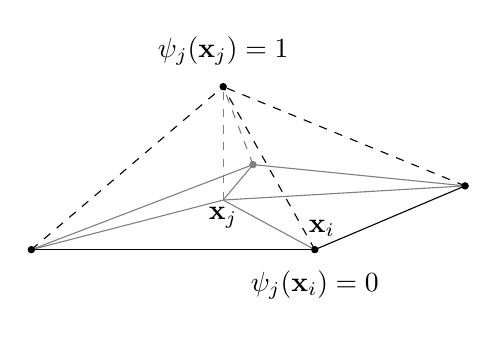
\begin{tikzpicture}[scale=0.9, z={(.707,.3)}]
    % (2,2,1) is top
    \draw[style=dashed] (0,0,0) -- (2,2,1); % to top from left
    \draw[style=dashed] (4,0,0) -- (2,2,1); %   ...  from front
    \draw[style=dashed] (4,0,3) -- (2,2,1); %   ...  from right
    \draw[color=gray, style=dashed] (0.3,0,4) -- (2,2,1); % from back
    \draw[color=gray, style=dashed] (2,0.4,1) -- (2,2,1); % from middle
    % draw base
    \draw (0,0,0) -- (4,0,0);
    \draw (4,0,0) -- (4,0,3);
    \draw[color=gray] (0,0,0) -- (0.3,0,4);
    \draw[color=gray] (0.3,0,4) -- (4,0,3);
    \draw[color=gray] (0,0,0) -- (2,0.4,1);
    \draw[color=gray] (2,0.4,1) -- (4,0,3);
    \draw[color=gray] (4,0,0) -- (2,0.4,1);
    \draw[color=gray] (2,0.4,1) -- (0.3,0,4);
    % draw \psi_j at nodes
    \filldraw (2,2,1) circle (1.25pt);
    \draw (2,2.5,1) node {$\psi_j(\bx_j)=1$};
    \draw (2,0.15,1) node {$\bx_j$};
    \filldraw (0,0,0) circle (1.25pt);
    \filldraw (4,0,0) circle (1.25pt);
    \draw (4,-0.5,0) node {$\psi_j(\bx_i)=0$};
    \draw (4.1,0.3,0) node {$\bx_i$};
    \filldraw (4,0,3) circle (1.25pt);
    \filldraw[color=gray] (0.3,0,4) circle (1.25pt);
\end{tikzpicture}


\caption{Hat functions $\psi_j$.}
\label{fig:un:hatfunction}
\end{marginfigure}

The FEM itself can now be stated.  It requires \eqref{eq:un:poissonweak} to be true for $u^h\in S_{g}^h$ for all $v^h\in S_{0}^h$.  However, it suffices to consider $v^h$ from a basis of $S_{0}^h$, so we require
\begin{equation}
\int_\Omega a(u^h) \grad u^h \cdot \grad \psi_i = \int_\Omega f(u^h) \psi_i + \int_{\partial_N\Omega} g_N \psi_i \label{eq:un:weakformhat}
\end{equation}
for all $i$ such that $\bx_i \notin \partial_D \Omega$.  On the other hand we may expand $u^h$ using $N-n_D$ unknown coefficients $u_j\in\RR$:
\begin{equation}
u^h(x,y) = \hat g_D(x,y) + \sum_{\bx_j \notin \partial_D \Omega} u_j\, \psi_j(x,y). \label{eq:un:uhexpand}
\end{equation}

The coefficients $u_j$ in \eqref{eq:un:uhexpand} are the unknowns.  Given the triangulation $\mathcal{T}_h$ of $\Omega$ and the data of the problem, namely the functions $a$, $f$, $g_D$, and $g_N$, the complete specification of the FEM solution $u^h$ is given by equations \eqref{eq:un:hatgdefine}, \eqref{eq:un:weakformhat}, and \eqref{eq:un:uhexpand}.

In the linear case it is common to now write system \eqref{eq:un:weakformhat} and \eqref{eq:un:uhexpand} as a linear system $A \bu = \bb$.  The usual next step in an FEM is to assemble the \emph{stiffness matrix} $A$ \citep{Elmanetal2005}.  However, we will not do so until we have an initial, and verified, numerical solution.  Following the pattern established since Chapter \ref{chap:nl}, we first implement equation \eqref{eq:un:weakformhat} as a residual-evaluation function $\bF(\bu)$, from the representation of $u^h$ as a vector $\bu$.  In evaluating $\bF$ we use \eqref{eq:un:uhexpand} to get point values of $u^h$ and its gradient $\grad u^h$ on the interior of triangles.  These point values allow quadrature, similar to that in Chapter \ref{chap:of}, to approximate the integrals in \eqref{eq:un:weakformhat}.  Implementing a residual in the linear case is mathematically equivalent to assembling $A$ and $\bb$, but the residual-evaluation code here is simpler because it does not require direct contact with a \pMat object at all.

In the next section we describe and the code the element-wise ``assembly,'' that is, evaluation of, the residual function $\bF$, as a \pSNES call-back.  However, before that can be written we need to be more specific about what \eqref{eq:un:weakformhat} says on each element.  Also we will read-in the triangular mesh and put it into \PETSc data structures.  These tools can be tested for correctness with a finite-differenced Jacobian (Chapter \ref{chap:nl}).  Once this is all shown to work correctly, via comparison to an exact solution, then we will re-consider matrix assembly, namely for the Jacobian derivative of $\bF$.


\section{Assembly of the residual equations}

Expression \eqref{eq:un:uhexpand} shows that $N-n_D$ real values $\{u_j\}$, for $j$ such that $\bx_j \notin \partial_D \Omega$, are needed to determine the FEM solution $u^h$.  However, it will be easier to write code if we \emph{increase} the size of the resulting nonlinear system, up to dimension $N$, by including the values of $u^h$ at nodes in the Dirichlet boundary as unknowns.  Thus we define
\begin{equation}
\bu = \{u_j\}_{j=0}^{N-1} \in \RR^N  \label{eq:un:unknowns}
\end{equation}
as the description of the FEM solution.

To enforce the boundary conditions, the components of the residual corresponding to Dirichlet boundary must be zero:
\begin{equation}
F_i(\bu) = u_i - g_D(\bx_i) \qquad \text{ if } \bx_i \in \partial_D\Omega.  \label{eq:un:dirichletresiduals}
\end{equation}

Because triangulation $\mathcal{T}_h$ satisfying \eqref{eq:un:triangulation} almost\sidenote{The set $\Omega \setminus \cup_k \triangle_k$ has measure zero.} covers $\Omega$ with non-overlapping triangles, we can write the weak form \eqref{eq:un:weakformhat} as a sum over elements.  To be specific, for each $\triangle_k \in \mathcal{T}_h$, $k=0,\dots,K-1$, let
\begin{equation}
F_i^k(\bu) = \int_{\triangle_k} a(u^h) \grad u^h \cdot \grad \psi_i - f(u^h) \psi_i.  \label{eq:un:elementweakform}
\end{equation}
Suppose $n_N$ is the number of edges which are in the Neumann boundary.  We call these edges (Neumann) \emph{segments} for distinctive language.  For each segment $s_\nu$, $\nu=0,\dots,n_N-1$, let
\begin{equation}
\varphi_i^\nu = \int_{s_\nu} g_N \psi_i,  \label{eq:un:segmentweakform}
\end{equation}
and note that $\varphi_i^\nu$ does not depend on the solution $u^h$.  Then residual equation \eqref{eq:un:weakformhat} is
\begin{equation}
F_i(\bu) = \sum_{k=0}^{K-1} F_i^k(\bu) - \sum_{\nu=0}^{n_N-1} \varphi_i^\nu = 0  \qquad \text{ if } \bx_i \notin \partial_D\Omega. \label{eq:un:elementwisesum}
\end{equation}
Together, equations \eqref{eq:un:dirichletresiduals} and \eqref{eq:un:elementwisesum} form the (generally) nonlinear system, of dimension $N$, which we supply to the \pSNES solver:
\begin{equation}
\bF(\bu)=0. \label{eq:un:fullsystem}
\end{equation}

Observe that $n_D$ is the number of \emph{nodes} in the Dirichlet boundary, whereas $n_N$ is the number of \emph{segments} (edges) in the Neumann boundary.  The former correspond to degrees of freedom, while the latter are domains of integration.  Managing the mesh correctly requires making this distinction.

Because the support of the hat function $\psi_i$ only overlaps with a few triangles $\triangle_k$, only a few values $F_i^k(\bu)$ and $\varphi_i^\nu$ are nonzero.  Also, only a few nodal values $\bu=\{u_j\}$ enter into $F_i^k(\bu)$, namely those values $u_j$ such that the support of $\psi_j$ overlaps with $\triangle_k$.  These facts make \eqref{eq:un:fullsystem} a \emph{sparse} nonlinear system.

We will compute the element integrals \eqref{eq:un:elementweakform} by referring $\triangle_k$ to a reference triangle $\triangle_\ast$ with vertices $(0,0),\,(1,0),\,(0,1)$, as shown in Figure \ref{fig:isoparametric}.  In Chapter \ref{chap:of} we did the same thing for quadrilaterals, so now we can be brief.

If $\triangle_k$ has vertices $(x_0,y_0),\,(x_1,y_1),\,(x_2,y_2)$ then the linear map from $\triangle_\ast$ to $\triangle_k$ is
\begin{align}
x(\xi,\eta) &= x_0 + (x_1-x_0) \xi + (x_2-x_0) \eta, \label{eq:un:trianglemap} \\
y(\xi,\eta) &= y_0 + (y_1-y_0) \xi + (y_2-y_0) \eta. \notag
\end{align}
The Jacobian determinant of map \eqref{eq:un:trianglemap}, needed for change-of-variables to integrate over the reference element, is constant on each element.  Its magnitude is the ratio of the area of $\triangle_k$ to the area of the reference element $\triangle_\ast$, equal to $2|\triangle_k|$ because $|\triangle_\ast|=1/2$.  See Exercise \ref{chap:un}.\ref{exer:un:gradientdetails}.

\begin{marginfigure}
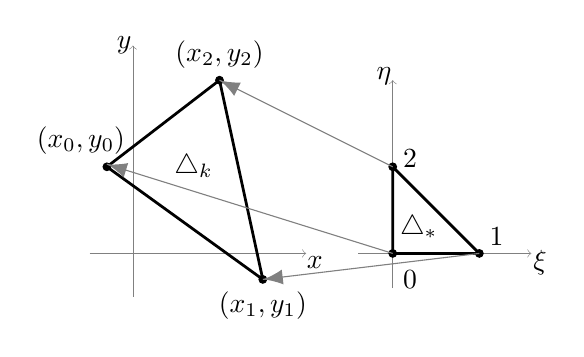
\begin{tikzpicture}[scale=1.1,
    decoration={
      markings,
      mark=at position 1 with {\arrow[scale=1.8,gray]{latex}};
    }]
% left x,y axes
    \draw[->, gray, very thin] (1.5,0) -- (4.0,0);
    \draw[->, gray, very thin] (2,-0.5) -- (2,2.4);
    \draw (4.1,-0.1) node {$x$};
    \draw (1.9,2.4) node {$y$};
    \filldraw (1.7,1) circle (1.25pt);    % (x_0,y_0)
    \filldraw (3.5,-0.3) circle (1.25pt); % (x_1,y_1)
    \filldraw (3.0,2.0) circle (1.25pt);  % (x_2,y_2)
    \draw (1.4,1.3) node {$(x_0,y_0)$};
    \draw (3.5,-0.6) node {$(x_1,y_1)$};
    \draw (3.0,2.3) node {$(x_2,y_2)$};
    \draw[line width=1pt] (1.7,1) -- (3.5,-0.3) -- (3.0,2.0) -- cycle;
    \draw (2.7,1.0) node {$\triangle_k$};
% right xi,eta axes
    \draw[->, gray, very thin] (4.6,0) -- (6.6,0);
    \draw[->, gray, very thin] (5,-0.4) -- (5,2.0);
    \draw (6.7,-0.1) node {$\xi$};
    \draw (4.9,2.05) node {$\eta$};
    \filldraw (5,0) circle (1.25pt);  % (0,0)
    \filldraw (6,0) circle (1.25pt);  % (1,0)
    \filldraw (5,1) circle (1.25pt);  % (0,1)
    \draw (5.2,-0.3) node {$0$};
    \draw (6.2,0.2) node {$1$};
    \draw (5.2,1.1) node {$2$};
    \draw[line width=1pt] (5,0) -- (6,0) -- (5,1) -- cycle;
    \draw (5.3,0.3) node {$\triangle_\ast$};
% arrows connecting nodes
    \draw[gray, postaction={decorate}] (5,0) -- (1.7,1.03);
    \draw[gray, postaction={decorate}] (6,0) -- (3.5,-0.3);
    \draw[gray, postaction={decorate}] (5,1) -- (3.0,2.0);
\end{tikzpicture}


\caption{Mapping of a triangle $\triangle_k$ from the reference triangle $\triangle_\ast$.}
\label{fig:isoparametric}
\end{marginfigure}

On $\triangle_\ast$ any linear function is a linear combination of three local (nodal) basis functions:
\begin{equation}
\chi_0(\xi,\eta) = 1-\xi-\eta, \qquad \chi_1(\xi,\eta) = \xi, \qquad \chi_2(\xi,\eta) = \eta. \label{eq:un:chiformulas}
\end{equation}
If $\bx_i\in\overline{\triangle_k}$ then hat function $\psi_i$ satisfies
\begin{equation}
\psi_i(x(\xi,\eta),y(\xi,\eta)) = \chi_\ell(\xi,\eta) \label{eq:un:psichimap}
\end{equation}
for all $(\xi,\eta)\in\triangle_\ast$, where vertex $\ell \in \{0,1,2\}$ of $\triangle_\ast$ maps to $\bx_i$.

Recalling both the change-of-variables formula for integrals and the chain rule, we can write
\begin{equation}
F_i^k(\bu) = 2 |\triangle_k| \int_{\triangle_\ast} H_\ell^k(\bu,\xi,\eta)\,d\xi\,d\eta \label{eq:un:elementintegralreference}
\end{equation}
where the integrand is
\begin{equation}
H_\ell^k(\bu,\xi,\eta) = \left[a(u^h) \grad u^h \cdot \grad \psi_i - f(u^h) \psi_i\right]_{\triangle_\ast}.  \label{eq:un:elementintegrand}
\end{equation}
Here vertex $\ell$ of $\triangle_\ast$ corresponds to the node $\bx_i$.  Note that ``$\grad$'' in \eqref{eq:un:elementintegrand} refers to derivatives in variables $x,y$.  Exercises \ref{chap:un}.\ref{exer:un:gradientdetails} and \ref{chap:un}.\ref{exer:un:elementintegranddetails} addresses the details implicit in \eqref{eq:un:elementintegralreference} and \eqref{eq:un:elementintegrand}.

As in Chapter \ref{chap:of}, the integrals \eqref{eq:un:elementintegralreference} will be approximated using quadrature.  Generally, if there are $Q$ quadrature points $(\xi_q,\eta_q) \in \triangle_\ast$ with weights $w_q$ then
\begin{equation}
F_i^k(\bu) \approx 2 |\triangle_k| \sum_{q=0}^{Q-1} w_q H_\ell^k(\bu,\xi_q,\eta_q). \label{eq:un:elementquadraturereference}
\end{equation}
We use symmetric quadrature rules constructed for the reference triangle $\triangle_\ast$.\sidenote{Unsymmetric quadrature rules based on tensor products of one-dimensional integrals \citep{KarniadakisSherwin2013} are an alternative.}  Table \ref{tab:un:quadrature} shows degree $1,2,3$ Gaussian rules \citep{Dunavant1985} with $Q=1,3,4$ points, respectively (Exercise \ref{chap:un}.\ref{exer:un:checkquadrature}).  Note that the sum of the weights is $1/2$ because $|\triangle_\ast|=1/2$.

\begin{table}[h]
\vspace{0.1in}

\begin{tabular}{lccc}
degree & $Q$ & weights $w_q$ & nodes $(\xi_q,\eta_q)$ \\ \hline
$1$ & $1$ & $1/2$ & $(1/3,1/3)$ \\ \hline
$2$ & $3$ & \begin{tabular}{c}
            $1/6$ \\
            $1/6$ \\
            $1/6$
            \end{tabular} & \begin{tabular}{c}
            $(1/6,1/6)$ \\
            $(2/3,1/6)$ \\
            $(1/6,2/3)$
            \end{tabular} \\ \hline
$3$ & $4$ & \begin{tabular}{c}
            $-27/96$ \\
            $25/96$ \\
            $25/96$ \\
            $25/96$
            \end{tabular} & \begin{tabular}{c}
            $(1/3,1/3)$ \\
            $(1/5,1/5)$ \\
            $(3/5,1/5)$ \\
            $(1/5,3/5)$
            \end{tabular}
\end{tabular}

\vspace{0.1in}
\caption{Symmetric quadrature rules on the reference triangle $\triangle_\ast$.  See \eqref{eq:un:elementquadraturereference}.} \label{tab:un:quadrature}
\end{table}

For the Neumann boundary contributions we use the midpoint rule.  Observe that hat function $\psi_i$ has value $1/2$ at the midpoint of any edge which is incident to $\bx_i$.  Thus
\begin{equation}
\varphi_i^\nu \approx g_N(x_m,y_m) \psi_i(x_m,y_m) |s_\nu| = \frac{1}{2} |s_\nu|\, g_N(x_m,y_m), \label{eq:un:segmentquadrature}
\end{equation}
if $\bx_i \in \overline{s_\nu}$, and it is zero otherwise.  Here $(x_m,y_m)$ is the midpoint, and $|s_\nu|$ is the length, of segment $s_\nu$.


\section{Example problems}

Let us set up some cases on a trapezoidal domain, with known exact solutions, for testing the FEM.  The first two cases are designed to test the implementation of the PDE and of Dirichlet boundary conditions.  One of these problems is linear and the other is nonlinear.  An additional case tests the non-homogeneous Neumann boundary condition implementation.  These cases are about as simple as possible given that they test the important parts of our code (below).  That is, we the errors from the FEM will only converge a the theoretical rate $O(h^2)$ if our implementation is correct.

All three cases are based on manufactured solutions.  Let
\begin{equation}
  u_{\text{exact}}(x,y) = 1 - y^2 - \frac{1}{4} y^4. \label{eq:un:exactsolution}
\end{equation}
This function also computes the Dirichlet boundary values $g_D(x,y)$ in all cases.  Because the domain is not aligned with the coordinate axes, and because fourth-order polynomials generate non-zero interpolation errors in a $P^1$ FEM, the numerical error generated with this exact solution will decay no more rapidly than the generic rate.

\begin{figure}
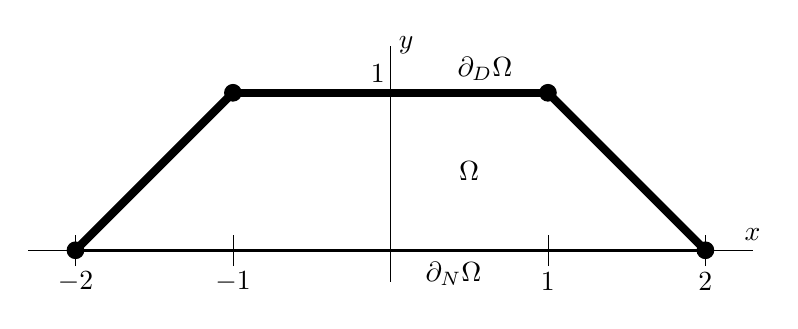
\begin{tikzpicture}[scale=2.000000]
% originally created, in part, by script tri2tikz.py command line:
%   tri2tikz.py --polyonly --nodesize 1.0 --scale 2.0 ../c/ch8/meshes/trap tmp/trap.tikz
% with by-hand edits
  \draw[thin] (0.0,-0.2) -- (0.0,1.3);
  \draw[thin] (-2.3,0.0) -- (2.3,0.0);
  \node at (2.3,0.1) {$x$};
  \node at (0.1,1.3) {$y$};
  \node at (0.5,0.5) {$\Omega$};
  \node at (-0.08,1.12) {$1$};
  \draw[very thin] (-2.0,-0.1) -- (-2.0,0.1);
  \node at (-2.0,-0.2) {$-2$};
  \draw[very thin] (-1.0,-0.1) -- (-1.0,0.1);
  \node at (-1.0,-0.2) {$-1$};
  \draw[very thin] (1.0,-0.1) -- (1.0,0.1);
  \node at (1.0,-0.2) {$1$};
  \draw[very thin] (2.0,-0.1) -- (2.0,0.1);
  \node at (2.0,-0.2) {$2$};
  \node at (0.4,-0.15) {$\partial_N \Omega$};
  \node at (0.6,1.15) {$\partial_D \Omega$};
  \draw[line width=3.0pt] (2.000000,0.000000) -- (1.000000,1.000000);
  \draw[line width=3.0pt] (1.000000,1.000000) -- (-1.000000,1.000000);
  \draw[line width=3.0pt] (-1.000000,1.000000) -- (-2.000000,0.000000);
  \draw[line width=1.25pt] (-2.000000,0.000000) -- (2.000000,0.000000);
  \filldraw (2.0,0.0) circle (1.5pt);
  \filldraw (1.0,1.0) circle (1.5pt);
  \filldraw (-1.0,1.0) circle (1.5pt);
  \filldraw (-2.0,0.0) circle (1.5pt);
\end{tikzpicture}

\caption{Exact solution cases $0$ and $1$ solve Poisson equations on a trapezoidal region $\Omega$.  Boundary subsets $\partial_D\Omega$, $\partial_N \Omega$ are as indicated.  See \texttt{trap.poly} in Code \ref{code:trappoly}.}
\label{fig:un:trap}
\end{figure}

Other details are case-specific:
\begin{itemize}
\item[case $0$:] \emph{Linear}.  Use Figure \ref{fig:un:trap} boundary conditions.  Noting $\partial u_{\text{exact}}/\partial n = \partial u_{\text{exact}}/\partial y = 0$ on the Neumann boundary $\partial_N \Omega$, where $y=0$, let $g_N=0$.  Let $a=1$ and determine $f$ by differentiating the exact solution: $f(x,y) = -\grad^2 u_{\text{exact}} = 2 + 3 y^2$.
\item[case $1$:] \emph{Nonlinear}.  Again use Figure \ref{fig:un:trap} boundary conditions and $g_N=0$.  However, let $a(u) = 1+u^2$ and compute the corresponding $f(u)$ by differentiation.
\item[case $2$:] \emph{Non-homogeneous Neumann}.  Use Figure \ref{fig:un:trapneu} boundary conditions.  Let $a$, $f$ be as in case $0$.  Determine the (non-zero) value $g_N$ by differentiating $u_{\text{exact}}$ along the Neumann boundary, a line segment with outward unit normal vector $\bn = \left<1/\sqrt{2},1/\sqrt{2}\right>$.
\end{itemize}
See \texttt{c/\CODELOC cases.h} (not shown) for all remaining details.

\begin{figure}
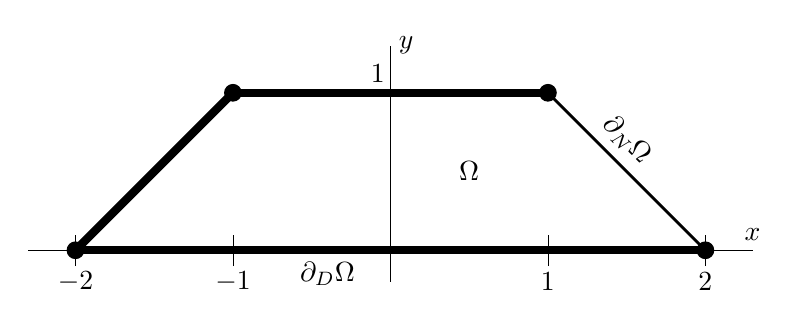
\begin{tikzpicture}[scale=2.000000]
% originally created, in part, by script tri2tikz.py command line:
%   tri2tikz.py --polyonly --nodesize 1.0 --scale 2.0 ../c/ch8/meshes/trap tmp/trap.tikz
% with by-hand edits
  \draw[thin] (0.0,-0.2) -- (0.0,1.3);
  \draw[thin] (-2.3,0.0) -- (2.3,0.0);
  \node at (2.3,0.1) {$x$};
  \node at (0.1,1.3) {$y$};
  \node at (0.5,0.5) {$\Omega$};
  \node at (-0.08,1.12) {$1$};
  \draw[very thin] (-2.0,-0.1) -- (-2.0,0.1);
  \node at (-2.0,-0.2) {$-2$};
  \draw[very thin] (-1.0,-0.1) -- (-1.0,0.1);
  \node at (-1.0,-0.2) {$-1$};
  \draw[very thin] (1.0,-0.1) -- (1.0,0.1);
  \node at (1.0,-0.2) {$1$};
  \draw[very thin] (2.0,-0.1) -- (2.0,0.1);
  \node at (2.0,-0.2) {$2$};
  \node at (-0.4,-0.15) {$\partial_D \Omega$};
  \node[rotate=-45] at (1.5,0.7) {$\partial_N \Omega$};
  \draw[line width=1.0pt] (2.000000,0.000000) -- (1.000000,1.000000);
  \draw[line width=3.0pt] (1.000000,1.000000) -- (-1.000000,1.000000);
  \draw[line width=3.0pt] (-1.000000,1.000000) -- (-2.000000,0.000000);
  \draw[line width=3.0pt] (-2.000000,0.000000) -- (2.000000,0.000000);
  \filldraw (2.0,0.0) circle (1.5pt);
  \filldraw (1.0,1.0) circle (1.5pt);
  \filldraw (-1.0,1.0) circle (1.5pt);
  \filldraw (-2.0,0.0) circle (1.5pt);
\end{tikzpicture}

\caption{Case $2$ uses the same region as in cases $0$ and $1$, but with different boundary conditions.  See \texttt{c/\CODELOC meshes/trapneu.poly} (not shown).}
\label{fig:un:trapneu}
\end{figure}


\section{Triangulations from \Triangle}

\PETSc does not include tools for triangulating regions of the plane, that is, for the initial generation of an unstructured mesh.  We use the widely-available \Triangle\sidenote{See \href{http://www.cs.cmu.edu/~quake/triangle.html}{www.cs.cmu.edu/$\sim$quake/ triangle.html} for documentation.} software \citep{Shewchuk1996} for this task.  \Triangle is limited to 2D, but the ASCII files it generates have straightforward details.

\Triangle inputs an ASCII file, with extension \texttt{.poly}, describing a polygonal region along with integer flags to indicate special vertices or segments on the boundary.  For example, the input file \texttt{trap.poly} (Code \ref{code:trappoly}) generates the polygon shown in Figure \ref{fig:un:trap}.

\inputwhole{../c/\CODELOC/meshes/trap.poly}{\CODELOC meshes/trap.poly}{A description of the boundary polygon in Figure \ref{fig:un:trap}, suitable for reading by \Triangle.}{code:trappoly}

The triangulation shown in Figure \ref{fig:un:trapone} came from applying \Triangle to \texttt{trap.poly}.  We ask for a polygon output file (option \texttt{-p}), relatively-uniform triangles (\texttt{-q} for ``quality-checked,'' with no interior angles less than $20^\circ$ \citep{Shewchuk1996}), and triangles with a maximum area (\texttt{-a}) of $0.5$:
\begin{cline}
$ cd c/ch7meshes
$ triangle -pqa0.5 trap
\end{cline}
%$
This command generates three ASCII files, \texttt{trap.1.node}, \texttt{trap.1.ele}, and \texttt{trap.1.poly}; see Codes \ref{code:traponenode}--\ref{code:traponepoly}.  They define the new node locations, elements as triples of node indices, and segments in the polynomial boundary as pairs of node indices, respectively.  This triangulation has $N=8$ nodes, $K=6$ elements, $P=8$ boundary segments, $n_D=5$ Dirichlet nodes, and $n_N=4$ segments in the Neumann boundary.

\begin{figure}
\input{tmp/trap.1.tikz}
\caption{The triangulation described by \texttt{trap.1.\{node,ele,poly\}}.}
\label{fig:un:trapone}
\end{figure}

By giving value ``$2$'' to the Dirichlet nodes in the original \texttt{trap.poly} input, and because \Triangle itself uses ``$0$'' for non-boundary and ``$1$'' for otherwise un-flagged boundary nodes, we have this boundary flag scheme:
\begin{itemize}
\item[0] interior node,
\item[1] Neumann boundary node or segment, and
\item[2] Dirichlet node or segment.
\end{itemize}
Observe that, though \texttt{trap.poly} describes the boundary using only 4 segments, additional boundary nodes and segments have been added in generating the triangulation.

\inputwhole{misc/trap.1.node}{\CODELOC meshes/trap.1.node}{\Triangle-generated ASCII file for node locations and nodal boundary flags.}{code:traponenode}

\inputwhole{misc/trap.1.ele}{\CODELOC meshes/trap.1.ele}{\Triangle-generated ASCII file with element index triples.}{code:traponeele}

\inputwhole{misc/trap.1.poly}{\CODELOC meshes/trap.1.poly}{\Triangle-generated ASCII file for the refined polygon, including segment boundary flags.}{code:traponepoly}

We will test the FEM on a sequence of refined grids generated by \Triangle.  For an example, the command
\begin{cline}
$ triangle -rpqa0.1 trap.1
\end{cline}
%$
generates ASCII files \texttt{trap.2.\{node,ele,poly\}} with $N=33$ nodes, $K=33$ elements, and $P=19$ boundary segments (Figure \ref{fig:un:traptwo}).  Refinement (\texttt{-r}) here means that \emph{nodes} in the \texttt{trap.1} files are retained, but there is no such inclusion relationship for the edges or triangles.  We also see that the symmetry of the \texttt{trap.1} mesh was merely fortuitous.  Symmetries in the input polygon are not preserved by the \Triangle algorithms.

\begin{figure}
\input{tmp/trap.2.tikz}
\caption{A refined triangulation.}
\label{fig:un:traptwo}
\end{figure}

\Triangle includes a minimal visualization tool.  The command
\begin{cline}
$ showme trap
\end{cline}
%$
displays the boundary polygon from \texttt{trap.poly} and levels of the triangulation (\texttt{trap.\{1,2\}.\{node,ele,poly\}}).


\section{From ASCII files to \PETSc \pVecs and \pISs}

Our plan is to traverse the lists of elements $\triangle_k \in \mathcal{T}_h$, and Neumann boundary segments $s_\nu$, so as to compute the residuals $F_i(\bu)$ from equations \eqref{eq:un:elementquadraturereference} and \eqref{eq:un:segmentquadrature}, respectively.  The traversal is fast if the mesh data are stored in \PETSc objects, so we first convert the above \Triangle-generated ASCII files into \pVecs and \pISs using a Python script \texttt{tri2petsc.py}.

An abstract description clarifies the data types.  There are two kinds of ``data'' to describe a mesh, \emph{geometrical} and \emph{topological}.  Here the geometry is simply the location, a pair of real numbers, for all the nodes.  For simplicity we store these $x$ and $y$ coordinates as separate length $N$ (sequential) \pVecs.  For the topology we need descriptions of which elements (triangles) are incident to which nodes (vertices).  This task only requires integer indices as we refer to a node simply by a global index into the coordinate \pVecs for $x$ and $y$.  Thus the topology of the elements is given by providing a triple of integers, in the range $0,\dots,N-1$, for each element.  Similarly, a segment of the polygonal boundary is simply a pair of nodal indices referring to the endpoints.

The \PETSc \pIS ``index set'' type is convenient for storing these indices.  The reader may regard an \pIS simply as an ``integer-valued \pVec'' in the current use.\sidenote{In this Chapter we do not exploit the ``main purpose'' of an \pIS in distributed (multi-process) indexing.}  The \pIS storing the element index triples holds $3K$ integers and the \pIS for boundary segments holds $2P$ integers.

Some care is needed in recording the Dirichlet and Neumann parts of the boundary.  First, one cannot tell if an edge in the triangulation is a boundary segment just from whether the endpoints are in the boundary.\sidenote{For example, the edge from node 5 to node 7 in Figure \ref{fig:un:number-mesh} is not a boundary segment.}  Second, the endpoints of a boundary segment could be nodes in the (closed) Dirchlet boundary, while the segment itself is in the (relatively-open) Neumann boundary.  Therefore, despite the apparent redundancy, we will separately store flags for the \emph{nodes}, indicating whether they are interior ($0$) or Neumann boundary ($1$) or Dirichlet boundary ($2$), and for the \emph{segments} on the boundary, either $1$ for Neumann or $2$ for Dirichlet.  This scheme is the one used by \Triangle.  Two more \pISs are used to store these flags.

Thus the Python script \texttt{tri2petsc.py} (not shown) reads three files in \Triangle-generated ASCII format, as described above, with extensions \texttt{.node,.ele,.poly}.  Then it writes two files in \PETSc binary format with extensions \texttt{.vec,.is}.  The first output file holds two \pVecs with the node coordinates.  The second output file holds four \pISs (element triples, nodal boundary flags, boundary segment pairs, and boundary segment flags).

Let's try it out.  Because \texttt{tri2petsc.py} uses Python modules from the \PETSc source directory, we first generate some symbolic links:
\begin{cline}
$ cd ..                                # back to c/ch7
$ ln -s ~/petsc/bin/petsc_conf.py
$ ln -s ~/petsc/bin/PetscBinaryIO.py
$ ./tri2petsc.py meshes/trap.1 trap.1
\end{cline}
This generates two files \texttt{trap.1.vec} and \texttt{trap.1.is}.  Our C code will then load these binary data with \PETSc functions  \texttt{VecLoad()} and \texttt{ISLoad()}, respectively.

It is convenient for the C code to have a data structure for all mesh information, so we define a new \texttt{UM} (``unstructured mesh'') data type, a C \texttt{struct}.  See Code \ref{code:umstruct}.  Of course, this \texttt{UM} data type is superceded by advanced, \PETSc-supported tools in Chapter \ref{chap:dp}.

\cinput{um.h}{\CODELOC}{An unstructured-mesh data type.}{//STARTUM}{//ENDUM}{code:umstruct}

Admittedly-tedious C functions \texttt{UMInitialize()}, \texttt{UMDestroy()}, \texttt{UMView()}, \texttt{UMReadVecs()}, and \texttt{UMReadISs()} in \texttt{c/\CODELOC um.c} (not shown) have the task of reading \texttt{.vec,.is} binary files and allocating/filling/destroying a \texttt{UM} instance.

\section{Initial implementation}

With an unstructured mesh in hand we can return to implementing the FEM.  We build the minimal \pSNES-using C code which works, called \texttt{c/\CODELOC unfem.c}.  In its initial implementation it has a ``context'' \texttt{struct}, which includes a \texttt{UM} instance, a residual-computation function \texttt{FormFunction()}, and a \texttt{main()} function.  The latter reads options and then creates\sidenote{And destroys at the end.} a \pSNES and \pVecs for holding the approximate solution, the exact solution, and the residual.  For the FEM itself we need enough information to transfer integrals to the reference triangle, and we need quadrature data structures, so we set these up.  There is then nothing else to do, other than to call \texttt{SNESSolve()}.  Figure \ref{fig:un:unfemstack} shows the structure of \texttt{unfem.c}, including the approximate Jacobian (implementation shown later).

Before showing this code, and because the reader might have become too comfortable with \pDMDA-using structured-grid examples in recent Chapters, recalling the first example in Chapter \ref{chap:nl} might be appropriate.  In terms of \PETSc objects and calls to the \PETSc API, \texttt{unfem.c} has a similar structure to \texttt{ecjac.c} in Chapter \ref{chap:nl}.

\begin{figure}
\begin{tikzpicture}[scale=0.8,
                    >={Latex[length=2mm]},
  component/.style={
     rectangle,draw,fill=white,align=center,line width=1pt},
  userfcn/.style={
     rounded corners,draw,fill=white,draw,align=center,line width=1pt,font={\itshape,\normalsize}}]

\draw[line width=1pt] (3,7) node[userfcn,minimum width=105mm] (usercode) {user code \\ \vspace{15mm}};

\draw[line width=1pt] (0,7.2) node[userfcn] (rescode) {residual \emph{\texttt{FormFunction()}}};
\draw[line width=1pt] (5.2,6.2) node[userfcn] (jaccode) {approximate Jacobian \emph{\texttt{FormPicard()}}};

\draw[line width=1pt] (-1,4) node[component] (snes) {\complabel{\pSNES}{nonlinear solver}};
\draw[line width=1pt] (-1,2) node[component] (ksp)  {\complabel{\pKSP}{linear solver}};
\draw[line width=1pt] (-1,0) node[component] (pc)   {\complabel{\pPC}{preconditioner}};

\draw[line width=1pt] (2,2) node[component] (matj)   {\usedlabel{\pMat}{Jacobian}};
\draw[line width=1pt] (3.5,0) node[component] (vecs)   {\pVecs \\ \footnotesize  \emph{solution, other fields}};
\draw[line width=1pt] (7.5,0) node[component] (iss)   {\pISs \\ \footnotesize  \emph{node indices, bdry flags}};

\path
   ([xshift=-10em]usercode.south) edge[->] node {} (snes)
   ([xshift=0em]usercode.south) edge[->] node {} ([xshift=2em]vecs.north)

   (rescode.south) edge[->,bend left] node {} (vecs.north)
   ([xshift=-2em]rescode.south) edge[->] node {} (iss.north)

   (jaccode.south) edge[->] node {} (matj)
   ([xshift=2em]jaccode.south) edge[->] node {} ([xshift=4em]vecs.north)
   ([xshift=4em]jaccode.south) edge[->] node {} ([xshift=2em]iss.north)

   (snes) edge node {} (ksp)
   (ksp) edge node {} (pc);
\end{tikzpicture}
\caption{The \PETSc object structure of \texttt{unfem.c}.}
\label{fig:un:unfemstack}
\end{figure}


FIXME show extracts of \texttt{main()} and most of \texttt{FormFunction()} in \texttt{c/\CODELOC unfem.c}


\section{Initial testing}

FIXME demo convergence with \texttt{-snes\_fd}


\section{Assembling an approximate Jacobian}

FIXME EXPLAIN PICARD $\bF(\bu)=0$ to $A(\bu) \bu - \bb(\bu)=0$ to $A(\bu^k) \bu^{k+1} - \bb(\bu^k)=0$ to $A(\bu^k) (\bu^{k+1}-\bu^k) - \bb(\bu^k)= - A(\bu^k) \bu^k$ to $A(\bu^k) \bs = -\bF(\bu^k)$  The linear system at a step, $A(\bu^k) \bs = -\bF(\bu^k)$, has $A=A(\bu^k)\in\RR^{N\times N}$ and $\bb=-\bF(\bu^k)\in\RR^N$, where $N$ is the number of nodes.  \pMat and \pVec objects store the problem, and, unlike in the \texttt{-snes\_fd} and \texttt{-snes\_mf} cases used above, wherein the \pMat object stayed invisibly inside the \pSNES solver, we now assemble the \pMat.

FIXME by considering \eqref{eq:un:dirichletresiduals}, \eqref{eq:un:elementweakform}, and \eqref{eq:un:elementwisesum}, the entries of this Picard/Jacobian matrix are
\begin{equation}
A_{ij}(\bu) =  \begin{cases}
               1, & i \in \partial_D\Omega \text{ or } j \in \partial_D\Omega, \\
               \sum_{k=0}^{K-1} A_{ij}^k(\bu), & \text{otherwise},
               \end{cases} \label{eq:un:picardentry}
\end{equation}
where
\begin{equation}
A_{ij}^k(\bu) = \int_{\triangle_k} a(u^h) \grad\psi_j \cdot \grad\psi_i \label{eq:un:picardentryelement}
\end{equation}
Again this is computed by quadrature, similar to \eqref{eq:un:elementintegralreference} and \eqref{eq:un:elementquadraturereference}.  This matrix is evidently symmetric, $a_{ij}=a_{ji}$, and sparse.  Furthermore it is positive-definite if $a(u,x,y)>0$, and thus the conjugate gradient Krylov method applies to the equations for the Newton step; see Chapter \ref{chap:ls}.

\section{Preallocate a \pMat (serial)}

FIXME essential for speed

compare for \texttt{--with-debugging=0} build:
\begin{cline}
$ timer ./unfem -un_mesh meshes/trap.7 -un_noprealloc
case 0 result for N=46421 nodes:  |u-u_exact|_inf = 6.55365e-05
real 56.30
$ timer ./unfem -un_mesh meshes/trap.7
case 0 result for N=46421 nodes:  |u-u_exact|_inf = 6.55365e-05
real 0.97
\end{cline}

\section{Performance relative to \pDMDA structured grid}

FIXME introduce \texttt{genstructured.py} and case 3; compares well in serial to Chapter 3 example

compare for \texttt{--with-debugging=0} build (note $1025^2=1050625$):
\begin{cline}
$ cd c/ch3/
$ make poisson
$ timer ./poisson -da_refine 7 -ksp_type cg -pc_type icc
on 1025 x 1025 grid:  error |u-uexact|_inf = 5.29691e-08
real 18.67
$ cd ../ch7
$ ./genstructured.py meshes/square.10 1025
$ ./tri2petsc.py meshes/square.10 meshes/square.10
$ make unfem
$ timer ./unfem -un_mesh meshes/square.10 -un_quaddeg 1 -un_case 3
case 3 result for N=1050625 nodes:  |u-u_exact|_inf = 9.89813e-08
real 24.47
\end{cline}

\section{Next steps}

FIXME: parallel approach could use \Triangle \texttt{.neigh} file as adjacency graph for elements, run \texttt{MatPartitioning} stuff (see manual), apply partitioning to get \pIS (or \texttt{AO}), and have nodes and edges follow along

FIXME: paraphrase Barry: The ``trick'' is that first partition the element across processes, then partition the vertices (nodal values) subordinate to the partitioning of the elements and then you renumber the elements and vertices so that the elements on the first process are numbered first, followed by the elements on the second process etc and similarly the vertices on the first process are numbered before the vertices on the second processes etc.  Each process loops over its elements computing the element stiffness/load and calling \texttt{MatSetValues/VecSetValues()} using the ``new'' numbering of the vertices.  The ``old'' numbering that was on the disk is not used in communicating with PETSc.

FIXME: see approach to mesh topology in chapter 10 of \citep{Loggetal2012}


\section{Exercises}

\renewcommand{\labelenumi}{\arabic{chapter}.\arabic{enumi}\quad}
\renewcommand{\labelenumii}{(\alph{enumii})}
\begin{enumerate}
\item  \label{exer:un:gradientdetails}  For the map \eqref{eq:un:trianglemap} from $\triangle_\ast$ to $\triangle_k$, let
    $$J_k = \frac{\partial (x,y)}{\partial (\xi,\eta)} = \begin{pmatrix}
    x_1 - x_0 & x_2 - x_0 \\
    y_1 - y_0 & y_2 - y_0 \end{pmatrix}
    = \begin{pmatrix}
    \Delta x_1 & \Delta x_2 \\
    \Delta y_1 & \Delta y_2
    \end{pmatrix}$$
be the Jacobian.  Use the chain rule and \eqref{eq:un:psichimap} to show that
\begin{equation}
\grad_{x,y} \psi_i = \frac{1}{\det J_k} \left<\Delta y_2 \frac{\partial \chi_\ell}{\partial \xi} - \Delta y_1 \frac{\partial \chi_\ell}{\partial \eta}, - \Delta x_2 \frac{\partial \chi_\ell}{\partial \xi} + \Delta x_1 \frac{\partial \chi_\ell}{\partial \eta}\right>. \label{eq:un:gradpsionref}
\end{equation}
Here indices $i$ and $\ell$ have the same relationship as in \eqref{eq:un:psichimap}.  Comparing formula \eqref{eq:of:gradpsionref} for the structured case, what is the underlying reason why \eqref{eq:un:gradpsionref} is a bit more complicated?  % underlying reason is that affine map here includes rotations, while in Chapter \ref{chap:of} it was just translation and axes scaling
\item  \label{exer:un:elementintegranddetails}  Formula \eqref{eq:un:elementintegrand} might require some interpretation before the implementation becomes clear.  Confirm that, with only mild abuses of notation, formulas \eqref{eq:un:trianglemap} and \eqref{eq:un:psichimap} lead to the valid expansions
\begin{align*}
a(u^h) &= a(u^h,\xi,\eta) = a(u^h,x(\xi,\eta),y(\xi,\eta)), \\
f(u^h) &= f(u^h,\xi,\eta) = f(u^h,x(\xi,\eta),y(\xi,\eta)), \\
\psi_i &= \chi_{\ell}(\xi,\eta), \\
u^h &= \sum_{j=0}^{N-1} \left\{\begin{matrix} g_D(\bx_j) \\ u_j \end{matrix}\right\} \chi_{\ell'}(\xi,\eta), \\
\grad u^h &= \grad_{x,y} u^h = \sum_{j=0}^{N-1} \left\{\begin{matrix} g_D(\bx_j) \\ u_j \end{matrix}\right\} \grad_{x,y} \psi_j.
\end{align*}
For the third formula, node $\bx_i$ corresponds to vertex $\ell$ on $\triangle_\ast$.  In the fourth and fifth formulas, node $\bx_j$ corresponds to vertex $\ell'$ on $\triangle_\ast$, and the two cases for the coefficient are when $\bx_j \in \partial_D \Omega$ and $\bx_j \notin \partial_D \Omega$, respectively.  Note that \eqref{eq:un:gradpsionref} allows us to expand $\grad_{x,y} \psi_j$ in the fifth formula.  Taken together, these expansions make \eqref{eq:un:elementintegrand} meaningful and implementable.
\item  \label{exer:un:checkquadrature}  The degree of accuracy $n=1,2,3$ of the quadrature rules in Table \ref{tab:un:quadrature} can be checked by comparing the exact integral
\begin{equation}
\iint_{\triangle_\ast} \xi^i \eta^j\,d\xi d\eta = \frac{i!\,j!}{(i+j+2)!}, \label{eq:un:checkquadrature}
\end{equation}
for all cases with $0\le i+j\le n$, against the quadrature result.  Also one should show an inexact quadrature result for some case with $i+j=n+1$.  Write a small program, in the language of your choice, which does these things.
\item \label{exer:un:basisfreeresidual} FIXME motivated by \citep{Loggetal2012}: replace $\bF(\bu)$ with $\bF(\bu;v)$ so that residual equation no longer requires basis of $S^h$ for its definition; advantages/disadvantages?
\item \label{exer:un:truejacobian} FIXME implement the true Jacobian in the $a=a(x,y)$ case, so that we only add a diagonal $\partial f/\partial u$ term; test on case 1 example and see if improved \pSNES convergence
\item \label{exer:un:bratu} FIXME using result from previous exercise, solve Bratu; compute critical $\lambda$; equals 6.81 according to \pSNES example \texttt{ex5.c}
\item \label{exer:un:gaussneumann}  In \texttt{unfem.c} we use the midpoint rule, the one-point Gauss rule, for quadrature \eqref{eq:un:segmentquadrature} computing the Neumann boundary segment contributions $\varphi_\nu^i$.  Modify \texttt{unfem.c} to optionally allow two-point Gaussian quadrature for this purpose.  Only in case 2 will this make any difference.  Show that accuracy improves for coarse grids, but that this benefit disappears under grid refinement.
% see c/ch7/solns/segmentgauss.c.snippet
\end{enumerate}

 % chapter 3


\chapter{Linear PDEs: multigrid}
\label{chap:multigrid}

We now make a transition from Chapters \ref{chap:structured} and \ref{chap:unstructured}.  In those chapters we wrote code to assemble the linear system for the problem on the grid or mesh initially chosen at runtime, and then we handed the system, in the form of \pMat and \pVec objects, to the \pKSP for solution.  In this Chapter, by contrast, we give a matrix-building code to \pKSP.  The \pKSP can actually choose the grid during the solution process, and ask our code (i.e.~through a ``call-back'') to assemble the matrix on that grid at that stage of the process.  This means \PETSc \pKSP object can do \emph{geometric multigrid} \citep{Briggsetal2000}.  To get started we recall basic ideas of multigrid.


\section{Multigrid basics}

FIXME: setup: suppose we are solving 1D Poisson equation on $\RR$, i.e.
    $$- u_{xx} = f(x)$$
with scheme
    $$- \frac{u_{j+1} - 2 u_j + u_{j-1}}{h^2} = f_j,$$
where $f_j = f(x_j)$, or equivalently
    $$- u_{j-1} + 2 u_j - u_{j+1} = h^2 f_j.$$

FIXME: idea (1) in 1D, on unbounded grid with spacing $h$, restriction to every other point takes lowish frequency wave to higher frequency wave on (still unbounded) grid with spacing $2h$

FIXME: idea (2) pointwise iteration version of Poisson FD scheme, e.g.~Jacobi
   $$u_j^{(m+1)} = \frac{1}{2} \left(u_{j-1}^{(m)} + u_{j+1}^{(m)} + h^2 f_j\right) $$
or Gauss-Seidel (where we update in increasing order on $j$)
   $$u_j^{(m+1)} = \frac{1}{2} \left(u_{j-1}^{(m+1)} + u_{j+1}^{(m)} + h^2 f_j\right) $$
will serve as low-pass filter on a given grid

FIXME: idea (3) given $u^{(0)}$ on fine $h$ grid, it is the residual FIXME

FIXME: for more, read \citep{Briggsetal2000} which is at same level as this book


\section{A multigrid-capable Poisson problem code}

Figure \ref{code:multigridone} show most of the code \texttt{c4poisson.c}.  Note the lines which create the \pKSP object and configure it:
\begin{code}
  KSP ksp;
  KSPCreate(PETSC_COMM_WORLD,&ksp);
  KSPSetDM(ksp,da);
  KSPSetComputeRHS(ksp,ComputeRHS,NULL);
  KSPSetComputeOperators(ksp,ComputeA,NULL);
  KSPSetFromOptions(ksp);
\end{code}
That is, we create \texttt{ksp} as in \texttt{c2poisson.c}, but this time we explicitly associate it to the \texttt{DM} object and then we hand it two methods \texttt{ComputeRHS()} and \texttt{ComputeA()} which it can call (i.e.~call back) when it needs the right-hand-side and the matrix of the system to be assembled.

\cinputpart{ch5poisson.c}{Poisson problem on a structured grid again, but this time using \texttt{KSPSetComputeOperators()} so that multigrid is possible.}{I}{//MAIN}{//ENDMAIN}{code:multigridone}

The code \texttt{c4poisson.c} is quite short because the two methods \texttt{ComputeRHS()} and \texttt{ComputeA()} are quite trivial ``wrappers'' around methods \texttt{formRHS()} and \texttt{formdirichletlaplacian()} from source file \texttt{structuredpoisson.c} in Chapter \ref{chap:structured}.  See Figure \ref{code:multigridtwo}.

\cinputpart{ch5poisson.c}{These methods build the right-hand side and the matrix, for call-back by \texttt{KSPSetComputeRHS()} and \texttt{KSPSetComputeOperators()}, respectively, but they are just wrappers around code reused from Chapter \ref{chap:structured}.}{II}{//COMPUTES}{//ENDCOMPUTES}{code:multigridtwo}

 % chapter 4


\section{Weak and strong scaling}

FIXME: define weak and strong scaling

FIXME: define arithmetic intensity

\section{Assessing our performance with event-logging and \texttt{-log\_summary}}

\vspace{4cm}

FIXME: also we can put a structured grid in the unstructured code

\begin{marginfigure}
\input{tmp/mesh.1.tikz}
\caption{A structured triangulation of the unit square with $K=32$ triangles and $N=25$ nodes.  The entire boundary is Dirichlet in the problem we consider.}
\label{fig:structuredfem}
\end{marginfigure}

FIXME: use CG and MG, and show cost of assembly

\section{Efficiency over mere scaling}

FIXME: how to show?

\section{Ideas}

FIXME: an idea that is most relevant to nonlinear problems: experimentation with linear solvers (i.e.~inside Newton) is obligatory because examples of linear systems can be found so that any solver comes out faster than any other \citep{Nachtigaletal1992} and examples of linear systems can be found so that well-known Krylov solvers like GMRES can be made to converge at any rate \citep{Greenbaumetal1996}

FIXME: perhaps discuss 64 bit PetscInt for large problems

FIXME: perhaps discuss PetscReal of \verb|__float128| for problems with large condition number where 64 bit \texttt{double} is not enough % chapter 5

%%%%%%%%%%

\chapter{6. Nonlinear elliptic PDEs on structured grids}

\section{Newton's method}

\section{\textsc{SNES}}
% c6newton.c

FIXME: somewhere in here we get to an idea that is most relevant to nonlinear problems: experimentation with linear solvers (i.e.~inside Newton) is obligatory because examples of linear systems can be found so that any solver comes out faster than any other \citep{Nachtigaletal1992} and examples of linear systems can be found so that well-known Krylov solvers like GMRES can be made to converge at any rate \citep{Greenbaumetal1996}

\section{Example: a porous medium equation}

\section{Jacobians: actual and approximate}

\caveat{But it isn't scaling well yet.}

%%%%%%%%%%

\chapter{7. More run-time preconditioner composition}

\section{Indeterminant systems: Stokes}

\section{More preconditioners}

\caveat{But \PETSc should help with unstructured meshes too.}

%%%%%%%%%%

\chapter{8. Unstructured grids, the right way}

\section{\textsc{DMPlex}}

\caveat{But my PDE isn't really a PDE.  It has an inequality in it.}

%%%%%%%%%%


\chapter{PDEs with constraints}
\label{chap:constrained}

\section{A variational inequality problem}

On a square $R = [-2,2]\times [-2,2]$.  Suppose $\psi \in H^1(R)$ has $\psi\big|_{\partial R} \le 0$ (in a trace sense).  Suppose we have $g\in L^2(\partial R)$ where $g \ge 0$ a.e.~on $\partial R$.  Consider the problem of finding $u\in H_0^1(R)$ so that
\begin{equation}
    \grad^2 u = 0 \text{ on } \{u > \psi\} \text{ \emph{and} } u\ge \psi. \label{obstaclestrong}
\end{equation}

This obstacle problem is nonlinear even though the Laplace equation is $\grad^2 u = 0$ is linear.

This obstacle problem is equivalent to minimization of the functional
\begin{equation}
I[u] = \frac{1}{2} \int_R \grad u\cdot \grad u
\end{equation}
over the constraint set
\begin{equation}
\mathcal{K} = \left\{u \in H_0^1(R) \,\Big|\, u\ge \psi\right\}.
\end{equation}

The code we write solves a problem where the exact solution is known for the given $\psi$ and boundary values in question.  In this case
   $$\psi(x,y) = \begin{cases} 1 - r^2, & r \le 1, \\  0, & \text{otherwise},\end{cases}$$
where, as expected, $r = (x^2+y^2)^{1/2}$.% FIXME: \psi is not in H^1, technically
Then the exact solution is
   $$u_{\text{exact}}(x,y) = \begin{cases} \psi(x,y), & r \le r_{\text{free}}, \\  - A \ln(r) + B, & \text{otherwise},\end{cases}$$
where $r_{\text{free}} = 0.69797$, $A = 0.68026$, and $B = 0.47152$.

\cinputpart{obstacle.c}{c/}{Just the struct.}{I}{//STRUCT}{//ENDSTRUCT}{code:obstaclestruct}

\cinputpart{obstacle.c}{c/}{Create the DMDA and Vecs.}{II}{//CREATE}{//ENDCREATE}{code:obstaclecreate}

\cinputpart{obstacle.c}{c/}{Setup the SNESVI object.}{III}{//SETUPSNES}{//ENDSETUPSNES}{code:obstaclesetupsnes}

\cinputpart{obstacle.c}{c/}{Compute the function $\psi$ and the exact solution, which determines the boundary conditions.}{IV}{//FORMPSI}{//ENDFORMPSI}{code:obstacleformpsi}

\cinputpart{obstacle.c}{c/}{From \PETSc 's point of view we are solving ``$F(u)=0$ subject to $u\ge \psi$''; this method computes $F(u)$.}{V}{//FORMFUNC}{//ENDFORMFUNC}{code:obstacleformfunc}

\cinputpart{obstacle.c}{c/}{This method assembles the Jacobian $J = F'(u)$.}{VI}{//FORMJAC}{//ENDFORMJAC}{code:obstacleformjac}

\cinputpart{obstacle.c}{c/}{An important part: tell SNESVI object about bound $u\ge \psi$ (and $u<+\infty$ because SNESVI expects both upper and lower bounds).}{VII}{//FORMBOUNDS}{//ENDFORMBOUNDS}{code:obstacleformbounds}

\cinputpart{obstacle.c}{c/}{Solve and report on results.}{VIII}{//SOLVE}{//ENDSOLVE}{code:obstaclesolve}

\section{Ice sheets}


%\section{General linear constraints}
%Date: Sat, 22 Aug 2015 21:29:25 -0500
%From: Barry Smith <bsmith@mcs.anl.gov>
%To: David Knezevic <david.knezevic@akselos.com>
%Cc: PETSc users list <petsc-users@mcs.anl.gov>
%Subject: Re: [petsc-users] Variatonal inequalities
%
%  David,
%
%   Currently the only way to do this without adding a lot of additional PETSc code is to add additional variables such that only box constraints appear in the final problem. For example say you have constraints   c <= Ax <= d then introduce new variables y = Ax and then you have the larger problem of unknowns (x,y) and box constrains on y with -infinity and +infinity constraints on x.
%
%  Barry
%
%> On Aug 22, 2015, at 6:59 AM, David Knezevic <david.knezevic@akselos.com> wrote:
%> Hi all,
%> I see from Section 5.7 of the manual that SNES supports box constraints on variables, which is great. However, I was also hoping to also be able to consider general linear inequality constraints, so I was wondering if anyone has any suggestions on how (or if) that could be done with PETSc?
%> Thanks,
%> David % chapter 9

%%%%%%%%%%

\backmatter

\bibliography{book}
\bibliographystyle{plainnat}

\clearpage

\newcommand{\tblockeqncode}[3]{
\begin{tabular}[t]{l} #1: \\ \qquad {\small #2} \\ \quad {\large \underline{\texttt{#3}}} \end{tabular}
}
\newcommand{\tblockcode}[2]{
\begin{tabular}[t]{l} #1 \\ \quad {\large \underline{\texttt{#2}}} \end{tabular}
}
\newcommand{\tblock}[1]{
\begin{tabular}[t]{l} #1 \end{tabular}
}

\thispagestyle{empty}
\noindent \textsc{inside front cover:}

\vfill
\begin{center}
\hspace{-10mm}\begin{tabular}{rllll}
\toprule
Chapter 
    &\quad linear\quad
          &linear
                &\quad nonlinear\quad
                      &nonlinear \\ 
    &     &time-dependent
                &     &time-dependent \\
\midrule  \bigskip
1   &     &     &     &      \\ \bigskip
2   & \tblockeqncode{Poisson}{$-\grad^2 u = f$}{c2poisson.c}
          & \tblockeqncode{heat}{$u_t = \grad^2 u$}{c2heat.c}
                &     &      \\ \bigskip
3   & \tblockcode{Poisson}{c3poisson.c}
          &     &     &      \\ \bigskip
4   & \begin{minipage}[t]{35mm}
 \tblockcode{Poisson}{c4poisson.c}

 \tblockeqncode{advection-diffusion}{$\bv \cdot \grad u - \grad^2 u = f$}{c4ad.c}
\end{minipage}
          &     &     &      \\ \bigskip
5   &     &     &     &      \\ \bigskip
6   &     &     & \tblockeqncode{$p$-Laplace}{$\begin{matrix} -\Div\left(D \grad u\right) = f \\ D = |\grad u|^{p-2} \end{matrix}$}{c6plap.c}
                      & \tblockeqncode{porous}{$\begin{matrix} u_t = \Div\left(D \grad u\right) \\ D = u^{\gamma-1} \end{matrix}$}{c6porous.c} \\ \bigskip
7   & \tblockeqncode{Stokes}{$\begin{matrix} \Div u = 0 \\ \grad p = \grad^2 u \end{matrix}$}{c7stokes.c}
          &     &     &      \\ \bigskip
8   & \tblockcode{Poisson}{c8poisson.c}
          &     &     &      \\
    & \tblockcode{Stokes}{c8stokes.c}
          &     &     &      \\ \bigskip
9   &     &     & \tblockeqncode{obstacle}{$\begin{matrix} -\grad^2 u = f \\ u\ge \psi \end{matrix}$}{c9obstacle.c}
                      & \tblockeqncode{ice sheet}{$\begin{matrix} H_t = \Div\left(D \grad H\right) + f \\ D = H^{n+2} |\grad (H-b)|^{n-1} \\ H \ge 0\end{matrix}$}{c9ice.c} \\
\bottomrule
\end{tabular}
\end{center}
\vfill


\newpage\thispagestyle{empty}
\noindent \textsc{inside back cover:}

\vfill
\begin{center}
\begin{tabular}{rccccccc}
\toprule
Chapter 
    &\;\pVec\; &\;\pMat\;
                &\;\pKSP\; &\pDMDA
                            &\pDMPlex
                                  &\pSNES &\;\pTS\; \\
\midrule
1   & \XX & \XX & \XX &     &     &     &      \\
2   & \XX & \XX & \XX & \XX &     &     & \XX  \\
3   & \XX & \XX & \XX &     &     &     &      \\
4   & \gX & \gX & \XX & \XX &     &     &      \\
5   & \gX & \gX & \XX & \XX &     &     &      \\
6   & \gX & \gX & \XX & \XX &     & \XX & \XX  \\
7   & \gX & \gX & \gX & \XX &     & \XX &      \\
8   & \gX & \gX & \XX &     & \XX & \XX &      \\
9   & \gX & \gX & \gX & \XX &     & \XX &      \\
\bottomrule
\end{tabular}
\end{center}
\vfill

\end{document}
